\documentclass[12pt, letterpaper]{article}
\usepackage[margin=1in]{geometry}
\usepackage[T1]{fontenc}
\usepackage{lmodern}
\usepackage{cmap}
\usepackage[utf8]{inputenc}
\usepackage{amsmath, amssymb, amsthm}
\usepackage{mathtools}
\usepackage{enumitem}
\usepackage{booktabs}
\usepackage{xcolor}
\usepackage{titlesec}
\usepackage{parskip}
\usepackage{hyperref}
\usepackage{fancyhdr}
\usepackage{tcolorbox}
\usepackage{graphicx}
\usepackage{caption}
\tcbuselibrary{skins, breakable}

\definecolor{darkblue}{RGB}{15,55,115}
\definecolor{midblue}{RGB}{30,100,180}
\definecolor{theorybg}{RGB}{245,250,255}
\definecolor{questionbg}{RGB}{255,252,240}
\definecolor{evencolor}{RGB}{60,0,100}

\hypersetup{colorlinks=true,linkcolor=darkblue,urlcolor=midblue,
  pdftitle={Ljungqvist and Sargent --- Recursive Macroeconomic Theory --- Complete Solutions, Chapter 2}}

\setlength{\headheight}{14pt}
\pagestyle{fancy}
\fancyhf{}
\renewcommand{\headrulewidth}{0.4pt}
\fancyhead[L]{\small\textcolor{darkblue}{\textit{Ljungqvist \& Sargent --- Recursive Macroeconomic Theory}}}
\fancyhead[R]{\small\textcolor{darkblue}{\thepage}}
\fancyfoot[C]{\small\textcolor{gray}{Complete Solutions --- Chapter 2}}

\titleformat{\section}[block]
  {\large\bfseries\color{darkblue}}{}{0pt}{}
  [\vspace{2pt}\color{darkblue}\rule{\textwidth}{1.5pt}\vspace{4pt}]

\titleformat{\subsection}[block]
  {\normalsize\bfseries\color{midblue}}{}{0pt}{}
  [\vspace{1pt}\color{midblue}\rule{0.5\textwidth}{0.8pt}\vspace{3pt}]

\tcbset{
  theorybox/.style={
    enhanced,breakable,colback=theorybg,colframe=darkblue,
    fonttitle=\bfseries\small\color{darkblue},boxrule=0.5pt,arc=3pt,
    left=6pt,right=6pt,top=4pt,bottom=4pt,title={Key Theory},
  },
  questionbox/.style={
    enhanced,breakable,colback=questionbg,colframe=gray!60,
    fonttitle=\bfseries\small\color{gray!60!black},boxrule=0.4pt,arc=2pt,
    left=6pt,right=6pt,top=4pt,bottom=4pt,title={\textit{Question}},
  },
  oddbox/.style={
    enhanced,breakable,colback=white,colframe=darkblue,
    attach boxed title to top left={yshift=-2mm,xshift=6mm},
    boxed title style={colback=darkblue,colframe=darkblue,arc=2pt,
      boxrule=0pt,left=6pt,right=6pt,top=3pt,bottom=3pt},
    fonttitle=\bfseries\large\color{white},
    boxrule=0.8pt,arc=3pt,
    left=8pt,right=8pt,top=10pt,bottom=6pt,
  },
  evenbox/.style={
    enhanced,breakable,colback=white,colframe=evencolor,
    attach boxed title to top left={yshift=-2mm,xshift=6mm},
    boxed title style={colback=evencolor,colframe=evencolor,arc=2pt,
      boxrule=0pt,left=6pt,right=6pt,top=3pt,bottom=3pt},
    fonttitle=\bfseries\large\color{white},
    boxrule=0.8pt,arc=3pt,
    left=8pt,right=8pt,top=10pt,bottom=6pt,
  },
  databox/.style={
    enhanced,breakable,colback=gray!8,colframe=gray!55,
    fonttitle=\bfseries\small\color{gray!60!black},boxrule=0.4pt,arc=2pt,
    left=6pt,right=6pt,top=4pt,bottom=4pt,title={Numerical exercise --- see the companion code},
  },
  trapbox/.style={
    enhanced,breakable,colback=red!4,colframe=red!45!black,
    fonttitle=\bfseries\small\color{white},boxrule=0.4pt,arc=2pt,
    coltitle=white,
    left=6pt,right=6pt,top=4pt,bottom=4pt,title={Where this goes wrong},
  },
}

\newcommand{\pd}[2]{\dfrac{\partial #1}{\partial #2}}
\newcommand{\dd}[2]{\dfrac{d #1}{d #2}}
\newcommand{\Var}{\mathrm{Var}}
\newcommand{\Cov}{\mathrm{Cov}}
\newcommand{\E}{E}
\newcommand{\tr}{\mathrm{trace}}
\newcommand{\yb}{\overline{y}}
\newcommand{\nb}[1]{\texttt{ls\_ch02.ipynb}, \S\,#1}

\setlist[enumerate,1]{label=(\alph*),itemsep=6pt,parsep=2pt}
\setlist[enumerate,2]{label=(\roman*),itemsep=3pt}

\begin{document}

%======================================================================
% TITLE PAGE
%======================================================================
\begin{titlepage}
\centering
\vspace*{2.5cm}
{\Huge\bfseries\color{darkblue} Recursive Macroeconomic Theory\par}
\vspace{6pt}
{\large Lars Ljungqvist and Thomas J.\ Sargent (4th ed., 2018)\par}
\vspace{1.4cm}
{\LARGE\bfseries Complete Solutions\par}
\vspace{6pt}
{\LARGE\bfseries Chapter 2 --- Time Series\par}
\vspace{1.2cm}
{\large All thirty end-of-chapter exercises, 2.1--2.30 (pp.~85--104)\par}
\vspace{2cm}

\begin{tcolorbox}[theorybox,title={What is in this file},width=0.86\textwidth]
\small
Every exercise carries the full question text, a step-by-step solution with no skipped
algebra, and a verification. Numerical answers are reproduced by the companion notebook
\texttt{Resolucao/ljungqvist\_sargent/ls\_ch02.ipynb}, which has one section per exercise and
checks every number against an independent route (closed form against recursion, truncated
sum, simulation, a Riccati solver, or brute-force Gaussian conditioning), aborting on any
mismatch. Where the book asks for Matlab (\texttt{doublej}, \texttt{bigshow3}, \texttt{kfilter})
the notebook does the same computation in Python.

\smallskip
Exercises are grouped by \textbf{topic}, not by number, following the order of the
chapter's own sections. Blue boxes are odd-numbered exercises, purple boxes even.

\smallskip
Ljungqvist--Sargent is supplementary reading and lies outside the course syllabus; this file is
for depth, not for the exam.
\end{tcolorbox}

\vfill
{\small MPE Insper --- Macroeconomia I --- 2026, 3\textordmasculine{} trimestre\par}
\end{titlepage}

\tableofcontents
\newpage

%======================================================================
\section{Chapter 2 \quad Time Series}
%======================================================================

\begin{tcolorbox}[theorybox,title={Chapter 2 Overview}]
The chapter builds two workhorse representations of a stochastic process and the tools that go
with them.

\smallskip
\textbf{Finite Markov chains} $(P,\pi_0)$. Distributions move by $\pi_{t+1}=P'\pi_t$; a stationary
distribution solves $(I-P')\pi=0$ (a left unit eigenvector); an invariant function solves
$(P-I)\yb=0$ (a right unit eigenvector, (2.2.13)). The chain is ergodic when every invariant
function is constant on the support of $\pi$, and then time averages converge to population
means (Theorem 2.2.5). Likelihoods factor as $\pi_{0,i_0}\prod_t P_{i_{t-1}i_t}$.

\smallskip
\textbf{Linear state-space systems} $x_{t+1}=Ax_t+Cw_{t+1}$, $y_t=Gx_t$. Means obey $\mu_{t+1}=A\mu_t$,
covariances $\Sigma_{t+1}=A\Sigma_tA'+CC'$ with stationary fixed point (2.4.10); forecasts are
$E_tx_{t+j}=A^jx_t$ and $E_t\sum\beta^jy_{t+j}=G(I-\beta A)^{-1}x_t$ (2.4.18); geometric sums of
quadratic forms solve the Lyapunov pair (2.4.20). The spectrum (2.11.2) is the Fourier transform of
the autocovariances.

\smallskip
\textbf{Hidden states.} When $y_t=Gx_t+v_t$ only is seen, the Kalman filter (2.7.14) is recursive
population regression; its time-invariant version gives the innovations representation (2.9.1) and
the VAR (2.9.3).

\smallskip
\textbf{Control.} Adding $u_t=-Fx_t$ turns (2.4.25) into policy evaluation and (2.4.30) into Howard
policy improvement; the LQ permanent income model (2.12.18) is the running application.
\end{tcolorbox}

%======================================================================
\subsection{Finite Markov Chains}
%======================================================================

%------- 2.1 -------
\begin{tcolorbox}[oddbox,title={Exercise 2.1 \quad Likelihood of Three Histories}]
\begin{tcolorbox}[questionbox]
Consider the Markov chain $(P,\pi_0)=\left(\begin{bmatrix}.9&.1\\.3&.7\end{bmatrix},
\begin{bmatrix}.5\\.5\end{bmatrix}\right)$, and a random variable $y_t=\yb x_t$ where
$\yb=\begin{bmatrix}1&5\end{bmatrix}$. Compute the likelihood of the following three histories
for $y_t$ for $t=0,1,\dots,4$:\\[3pt]
(a) $1,5,1,5,1$.\quad (b) $1,1,1,1,1$.\quad (c) $5,5,5,5,5$.
\end{tcolorbox}

\textbf{Solution:}

Because $\yb$ has distinct entries, each value of $y_t$ identifies the state ($y=1\Leftrightarrow
e_1$, $y=5\Leftrightarrow e_2$), so the likelihood of $y_0,\dots,y_4$ is the probability of the
state path:
\[
f(y_4,\dots,y_0)=\pi_{0,i_0}\,P_{i_0i_1}P_{i_1i_2}P_{i_2i_3}P_{i_3i_4}.
\]
\begin{enumerate}
\item Path $1,2,1,2,1$: $\;.5\times P_{12}P_{21}P_{12}P_{21}=.5\times.1\times.3\times.1\times.3
=.5\times.0009=\boxed{.00045}$.
\item Path $1,1,1,1,1$: $\;.5\times P_{11}^4=.5\times .9^4=.5\times .6561=\boxed{.32805}$.
\item Path $2,2,2,2,2$: $\;.5\times P_{22}^4=.5\times .7^4=.5\times .2401=\boxed{.12005}$.
\end{enumerate}
\emph{Reading.} The chain is persistent (large diagonal), so constant histories are far more likely
than alternating ones; state 1 is stickier than state 2 ($.9>.7$), so (b) beats (c).

\textbf{Verification.} \nb{2.1} recomputes all three with the forward recursion
$\alpha_t'=(\alpha_{t-1}'P)\odot\mathbf 1\{y_t\}$. \checkmark
\end{tcolorbox}

%------- 2.2 -------
\begin{tcolorbox}[evenbox,title={Exercise 2.2 \quad Recovering $P$ from Conditional Moments}]
\begin{tcolorbox}[questionbox]
Consider a two-state Markov chain. Consider a random variable $y_t=\yb x_t$ where
$\yb=\begin{bmatrix}1\\5\end{bmatrix}$. It is known that
$E(y_{t+1}|x_t)=\begin{bmatrix}1.8\\3.4\end{bmatrix}$ and that
$E(y^2_{t+1}|x_t)=\begin{bmatrix}5.8\\15.4\end{bmatrix}$. Find a transition matrix consistent with these
conditional expectations. Is this transition matrix unique (i.e., can you find another one that is
consistent with these conditional expectations)?
\end{tcolorbox}

\textbf{Solution:}

Conditional on $x_t=e_i$, $E(y_{t+1}|x_t)=\sum_jP_{ij}\yb_j$, i.e.\ the vector of conditional
means is $P\yb$; likewise the conditional second moments are $P\yb^{2}$ with $\yb^2=[1,25]'$.
Row $i$ has two unknowns and satisfies
\[
P_{i1}+P_{i2}=1,\qquad P_{i1}+5P_{i2}=m_i\;\Rightarrow\;1+4P_{i2}=m_i\;\Rightarrow\;P_{i2}=\frac{m_i-1}{4}.
\]
Row 1: $P_{12}=\frac{1.8-1}{4}=.2$, $P_{11}=.8$. Row 2: $P_{22}=\frac{3.4-1}{4}=.6$, $P_{21}=.4$.
\[
\boxed{P=\begin{bmatrix}.8&.2\\.4&.6\end{bmatrix}}
\]
Check the second moments: row 1: $.8(1)+.2(25)=.8+5=5.8$ \checkmark; row 2: $.4(1)+.6(25)=.4+15=15.4$ \checkmark.

\textbf{Uniqueness.} Yes, $P$ is unique. For each row the two equations (adding-up and the first
moment) have coefficient matrix $\begin{bmatrix}1&1\\1&5\end{bmatrix}$, with determinant $4\neq0$,
so they already pin the row down. The second-moment restriction is an \emph{overidentifying}
restriction: it could have been violated, and it is not.

\textbf{Verification.} \nb{2.2} stacks all six equations in the four unknowns: rank 4, zero
residual, and rank 4 still holds without the second-moment rows. \checkmark
\end{tcolorbox}

%------- 2.3 -------
\begin{tcolorbox}[oddbox,title={Exercise 2.3 \quad Discounted Utility and Bayesian Model Choice}]
\begin{tcolorbox}[questionbox]
Consumption is governed by an $n$-state Markov chain $P,\pi_0$ where $P$ is a stochastic matrix and
$\pi_0$ is an initial probability distribution. Consumption takes one of the values in the $n\times1$
vector $\overline c$. A consumer ranks stochastic processes of consumption $t=0,1,\dots$ according to
$E\sum_{t=0}^\infty\beta^tu(c_t)$ where $E$ is the mathematical expectation and
$u(c)=\frac{c^{1-\gamma}}{1-\gamma}$ for some parameter $\gamma\ge1$. Let $u_i=u(\overline c_i)$. Let
$v_i=E[\sum_{t=0}^\infty\beta^tu(c_t)|x_0=\overline e_i]$ and $V=Ev$, where $\beta\in(0,1)$ is a
discount factor.\\[3pt]
(a) Let $u$ and $v$ be the $n\times1$ vectors whose $i$th components are $u_i$ and $v_i$,
respectively. Verify the following formulas for $v$ and $V$: $v=(I-\beta P)^{-1}u$, and
$V=\sum_i\pi_{0,i}v_i$.\\
(b) Consider the following two Markov processes:
Process 1: $\pi_0=\begin{bmatrix}.5\\.5\end{bmatrix}$, $P=\begin{bmatrix}1&0\\0&1\end{bmatrix}$.
Process 2: $\pi_0=\begin{bmatrix}.5\\.5\end{bmatrix}$, $P=\begin{bmatrix}.5&.5\\.5&.5\end{bmatrix}$.
For both Markov processes, $\overline c=\begin{bmatrix}1\\5\end{bmatrix}$. Assume that
$\gamma=2.5,\beta=.95$. Compute the unconditional discounted expected utility $V$ for each of these
processes. Which of the two processes does the consumer prefer? Redo the calculations for
$\gamma=4$. Now which process does the consumer prefer?\\
(c) An econometrician observes a sample of 10 observations of consumption rates for our consumer. He
knows that one of the two preceding Markov processes generates the data, but he does not know
which one. He assigns equal ``prior probability'' to the two chains. Suppose that the 10 successive
observations on consumption are as follows: $1,1,1,1,1,1,1,1,1,1$. Compute the likelihood of this
sample under process 1 and under process 2. Denote the likelihood function
$\text{Prob}(\text{data}|\text{Model}_i)$, $i=1,2$.\\
(d) Suppose that the econometrician uses Bayes' law to revise his initial probability estimates
for the two models, where in this context Bayes' law states:
$\text{Prob}(M_i)|\text{data}=\frac{\text{Prob}(\text{data})|M_i\cdot\text{Prob}(M_i)}
{\sum_j\text{Prob}(\text{data})|M_j\cdot\text{Prob}(M_j)}$ where $M_i$ denotes model $i$. The
denominator of this expression is the unconditional probability of the data. After observing the
data sample, what probabilities does the econometrician place on the two possible models?\\
(e) Repeat the calculation in part d, but now assume that the data sample is
$1,5,5,1,5,5,1,5,1,5$.
\end{tcolorbox}

\textbf{Solution:}

\begin{enumerate}
\item Since $E[u(c_t)|x_0=e_i]=\sum_j(P^t)_{ij}u_j=(P^tu)_i$,
\[
v=\sum_{t=0}^\infty\beta^tP^tu=(I-\beta P)^{-1}u,
\]
where the geometric series converges because every eigenvalue of the stochastic matrix $P$ has
modulus $\le1$, so the spectral radius of $\beta P$ is $\beta<1$. Equivalently, splitting off
$t=0$ and using the Markov property,
$v_i=u_i+\beta\sum_jP_{ij}v_j$, i.e.\ $v=u+\beta Pv$, i.e.\ $(I-\beta P)v=u$. Finally, by the law of
iterated expectations over the initial state,
$V=E\,v(x_0)=\sum_i\pi_{0,i}v_i$. \checkmark

\item \emph{Process 1} ($P=I$): $v=(1-\beta)^{-1}u$, so $V_1=\dfrac{.5u_1+.5u_2}{1-\beta}$.

\emph{Process 2} ($P=\tfrac12\mathbf 1\mathbf 1'$): $P^tu=\bar u\,\mathbf 1$ for $t\ge1$, with
$\bar u\equiv .5u_1+.5u_2$. Hence $v=u+\frac{\beta}{1-\beta}\bar u\,\mathbf 1$ and
\[
V_2=\bar u+\frac{\beta}{1-\beta}\bar u=\frac{\bar u}{1-\beta}=V_1 .
\]
The two values are \textbf{identical for every $u$}, hence for every $\gamma$. Numbers:

$\gamma=2.5$: $u(1)=\frac{1}{-1.5}=-.666667$, $u(5)=\frac{5^{-1.5}}{-1.5}=\frac{.0894427}{-1.5}=-.0596285$;
$\bar u=-.363148$; $V_1=V_2=\frac{-.363148}{.05}=\boxed{-7.262951}$.

$\gamma=4$: $u(1)=-\frac13$, $u(5)=\frac{5^{-3}}{-3}=-.0026667$; $\bar u=-.168$;
$V_1=V_2=\frac{-.168}{.05}=\boxed{-3.36}$.

The consumer is \textbf{indifferent} in both cases.

\emph{Reading.} Both chains start from $[.5,.5]$, which is stationary for both, so in every period
$c_t$ equals 1 or 5 with probability one half under either process. Time-separable expected utility
only sees these period-by-period marginals, so it is blind to the serial correlation: a single coin
flip at $t=0$ fixing consumption for life (process 1) is valued exactly like a fresh flip every
period (process 2). Raising $\gamma$ changes the level of $V$, never the ranking.

\item The observations identify the states. Process 1: $\pi_{0,1}\cdot1^9=\boxed{.5}$.
Process 2: $.5\times.5^9=.5^{10}=\frac{1}{1024}=\boxed{.000977}$.

\item With equal priors the priors cancel:
\[
\text{Prob}(M_1|\text{data})=\frac{.5}{.5+.5^{10}}=\frac{512}{513}=\boxed{.998051},\quad
\text{Prob}(M_2|\text{data})=\boxed{.001949}.
\]
\item Process 1 has $P_{12}=0$: a switch from 1 to 5 has probability zero, so
$\text{Prob}(\text{data}|M_1)=0$, while $\text{Prob}(\text{data}|M_2)=.5^{10}$. Hence
$\boxed{\text{Prob}(M_1|\text{data})=0,\ \text{Prob}(M_2|\text{data})=1}$: a single switch refutes
process 1.
\end{enumerate}

\textbf{Verification.} \nb{2.3}: $(I-\beta P)^{-1}u$ against the truncated sum
$\sum_{t\le3000}\beta^tP^tu$; the likelihoods by the forward recursion. \checkmark
\end{tcolorbox}

\begin{tcolorbox}[trapbox]
It is tempting to say the risk-averse consumer ``must'' dislike the fully persistent process 1
because it is riskier over a lifetime. With time-separable utility and no way to save, lifetime
risk is irrelevant: only the distribution of $c_t$ at each date enters $V$. Preferring early or
late resolution of risk, or disliking persistence, requires non-separable (e.g.\ recursive)
preferences.
\end{tcolorbox}

%------- 2.10 -------
\begin{tcolorbox}[evenbox,title={Exercise 2.10 \quad Convex Combinations of Stationary Distributions}]
\begin{tcolorbox}[questionbox]
Let $P$ be a transition matrix for a Markov chain. Suppose that $P'$ has two distinct eigenvectors
$\pi_1,\pi_2$ corresponding to unit eigenvalues of $P'$. Scale $\pi_1$ and $\pi_2$ so that they are
vectors of probabilities (i.e., elements are nonnegative and sum to unity). Prove for any
$\alpha\in[0,1]$ that $\alpha\pi_1+(1-\alpha)\pi_2$ is an invariant distribution of $P$.
\end{tcolorbox}

\textbf{Solution:}

Let $\pi_\alpha=\alpha\pi_1+(1-\alpha)\pi_2$. Three things must hold.
\begin{enumerate}[label=(\roman*)]
\item \emph{Invariance.} By linearity and $P'\pi_k=\pi_k$:
$P'\pi_\alpha=\alpha P'\pi_1+(1-\alpha)P'\pi_2=\alpha\pi_1+(1-\alpha)\pi_2=\pi_\alpha$.
\item \emph{Nonnegativity.} Each entry is $\alpha\pi_{1,i}+(1-\alpha)\pi_{2,i}\ge0$, a combination with
nonnegative weights of nonnegative numbers.
\item \emph{Adding up.} $\mathbf 1'\pi_\alpha=\alpha\mathbf 1'\pi_1+(1-\alpha)\mathbf 1'\pi_2=\alpha+1-\alpha=1$.
\end{enumerate}
So $\pi_\alpha$ is a probability vector satisfying $\pi_\alpha=P'\pi_\alpha$, i.e.\ a stationary
(invariant) distribution. $\blacksquare$ The set of stationary distributions is therefore convex, as
the Remark after Definition 2.2.3 states; $\pi_1,\pi_2$ are its extreme points.

\textbf{Verification.} \nb{2.10} checks five values of $\alpha$ for a block-diagonal chain. \checkmark
\end{tcolorbox}

%------- 2.11 -------
\begin{tcolorbox}[oddbox,title={Exercise 2.11 \quad Transient Distribution of an Absorbing Chain}]
\begin{tcolorbox}[questionbox]
Consider a Markov chain with transition matrix
$P=\begin{bmatrix}1&0&0\\.2&.5&.3\\0&0&1\end{bmatrix}$ with initial distribution
$\pi_0=[\pi_{1,0}\ \pi_{2,0}\ \pi_{3,0}]'$. Let $\pi_t=[\pi_{1t}\ \pi_{2t}\ \pi_{3t}]'$ be the distribution
over states at time $t$. Prove that for $t>0$
\[
\pi_{1t}=\pi_{1,0}+.2\left(\frac{1-.5^t}{1-.5}\right)\pi_{2,0},\quad
\pi_{2t}=.5^t\pi_{2,0},\quad
\pi_{3t}=\pi_{3,0}+.3\left(\frac{1-.5^t}{1-.5}\right)\pi_{2,0}.
\]
\end{tcolorbox}

\textbf{Solution:}

The law of motion $\pi_{t+1}=P'\pi_t$ reads, component by component,
\[
\pi_{1,t+1}=\pi_{1t}+.2\pi_{2t},\qquad \pi_{2,t+1}=.5\pi_{2t},\qquad \pi_{3,t+1}=.3\pi_{2t}+\pi_{3t}.
\]
\emph{State 2.} The middle equation is a first-order linear difference equation:
$\pi_{2t}=.5\,\pi_{2,t-1}=\dots=.5^t\pi_{2,0}$.

\emph{State 1.} Summing the first equation from $0$ to $t-1$ and substituting $\pi_{2s}=.5^s\pi_{2,0}$:
\[
\pi_{1t}=\pi_{1,0}+.2\sum_{s=0}^{t-1}\pi_{2s}=\pi_{1,0}+.2\,\pi_{2,0}\sum_{s=0}^{t-1}.5^s
=\pi_{1,0}+.2\left(\frac{1-.5^t}{1-.5}\right)\pi_{2,0}.
\]
\emph{State 3.} Identically, with $.3$ in place of $.2$. $\blacksquare$

As $t\to\infty$: $\pi_{1\infty}=\pi_{1,0}+.4\pi_{2,0}$, $\pi_{2\infty}=0$,
$\pi_{3\infty}=\pi_{3,0}+.6\pi_{2,0}$. The mass initially in the transient state 2 is split between
the two absorbing states in the ratio $.2:.3$.

\textbf{Verification.} \nb{2.11}: iteration of $P'$ against the formulas for $t=1,\dots,39$. \checkmark
\end{tcolorbox}

%------- 2.12 -------
\begin{tcolorbox}[evenbox,title={Exercise 2.12 \quad Columns of $(P')^t$}]
\begin{tcolorbox}[questionbox]
Let $P$ be a transition matrix for a Markov chain. For $t=1,2,\dots$, prove that the $j$th column of
$(P')^t$ is the distribution across states at $t$ when the initial distribution is $\pi_{j,0}=1$,
$\pi_{i,0}=0\ \forall i\neq j$.
\end{tcolorbox}

\textbf{Solution:}

By the law of total probability and the Markov property,
$\text{Prob}(x_{t+1}=e_i)=\sum_k\text{Prob}(x_t=e_k)P_{ki}$, i.e.\ $\pi_{t+1}=P'\pi_t$. By induction,
$\pi_t=(P')^t\pi_0$: true at $t=1$, and if $\pi_t=(P')^t\pi_0$ then $\pi_{t+1}=P'(P')^t\pi_0=(P')^{t+1}\pi_0$.
With $\pi_0=e_j$, $\pi_t=(P')^te_j$, and post-multiplying a matrix by $e_j$ selects its $j$th column.
$\blacksquare$ Equivalently: $\big((P')^t\big)_{ij}=(P^t)_{ji}=\text{Prob}(x_t=e_i|x_0=e_j)$.

\textbf{Verification.} \nb{2.12}: columns against iteration, and a 200{,}000-path simulation. \checkmark
\end{tcolorbox}

%------- 2.14 -------
\begin{tcolorbox}[evenbox,title={Exercise 2.14 \quad A Reducible Four-State Chain}]
\begin{tcolorbox}[questionbox]
Consider a Markov chain with transition matrix
$P=\begin{bmatrix}.5&.5&0&0\\.1&.9&0&0\\0&0&.9&.1\\0&0&0&1\end{bmatrix}$ with state space
$X=\{e_i,i=1,\dots,4\}$ where $e_i$ is the $i$th unit vector. A random variable $y_t$ is a function
$y_t=[1\ 2\ 3\ 4]x_t$ of the underlying state.\\[3pt]
(a) Find all stationary distributions of the Markov chain.\\
(b) Can you find a stationary distribution for which the Markov chain is ergodic?\\
(c) Compute all possible limiting values of the sample mean $\frac1T\sum_{t=0}^{T-1}y_t$ as
$T\to\infty$.
\end{tcolorbox}

\textbf{Solution:}

\begin{enumerate}
\item Write $\pi=P'\pi$ component by component:
\[
\pi_1=.5\pi_1+.1\pi_2,\quad \pi_2=.5\pi_1+.9\pi_2,\quad \pi_3=.9\pi_3,\quad \pi_4=.1\pi_3+\pi_4 .
\]
The first gives $.5\pi_1=.1\pi_2\Rightarrow\pi_2=5\pi_1$ (the second says the same); the third gives
$\pi_3=0$; the fourth then holds for any $\pi_4$. With adding up, $6\pi_1+\pi_4=1$. Setting
$\alpha=6\pi_1$:
\[
\boxed{\pi_\alpha=\alpha\begin{bmatrix}1/6\\5/6\\0\\0\end{bmatrix}+(1-\alpha)\begin{bmatrix}0\\0\\0\\1\end{bmatrix},\qquad \alpha\in[0,1].}
\]
There are two closed classes, $\{1,2\}$ and $\{4\}$; state 3 is transient (it leaks into 4).

\item Yes: $\alpha=1$ or $\alpha=0$ (the two extreme points). For $\alpha\in(0,1)$ the function
$\yb=[1,1,0,0]'$ satisfies $P\yb=\yb$, so it is invariant, yet it is not constant on the support
$\{1,2,4\}$ of $\pi_\alpha$: the chain is not ergodic.

\item The limit depends on where the chain starts:
\begin{itemize}
\item $x_0\in\{e_1,e_2\}$: the chain stays in $\{1,2\}$, which is ergodic under $[1/6,5/6]$, so by
Theorem 2.2.5 the mean converges to $1\cdot\frac16+2\cdot\frac56=\boxed{\tfrac{11}{6}}$.
\item $x_0\in\{e_3,e_4\}$: state 3 is left for 4 with probability one (after a geometric time with mean
10), and 4 is absorbing, so the mean converges to $\boxed{4}$.
\end{itemize}
Drawing $x_0$ from $\pi_\alpha$, the limit is the random variable $E[y_\infty|x_0]$ of (2.2.11):
$11/6$ with probability $\alpha$ and $4$ with probability $1-\alpha$.
\end{enumerate}

\textbf{Verification.} \nb{2.14}: sample means over $200{,}000$ periods from each starting state:
$1.8341,\,1.8327,\,3.9999,\,4.0000$. \checkmark
\end{tcolorbox}

%------- 2.16 -------
\begin{tcolorbox}[evenbox,title={Exercise 2.16 \quad Law of Large Numbers for Indicators}]
\begin{tcolorbox}[questionbox]
Consider an $n$-state Markov chain with state space $X=\{e_i,i=1,\dots,n\}$ where $e_i$ is the $i$th
unit vector. Consider the indicator variable $I_{it}=e_ix_t$ which equals 1 if $x_t=e_i$ and 0
otherwise. Suppose that the chain has a unique stationary distribution and that it is ergodic. Let
$\pi$ be the stationary distribution.\\[3pt]
(a) Verify that $EI_{it}=\pi_i$.\\
(b) Prove that $\frac1T\sum_{t=0}^{T-1}I_{it}=\pi_i$ as $T\to\infty$ with probability one with respect
to the stationary distribution $\pi$.
\end{tcolorbox}

\textbf{Solution:}

\begin{enumerate}
\item $I_{it}$ is Bernoulli, so $EI_{it}=\text{Prob}(x_t=e_i)=\big((P')^t\pi\big)_i=\pi_i$, because
$x_0\sim\pi$ and $P'\pi=\pi$ make the distribution of $x_t$ equal to $\pi$ at every $t$.
\item $I_{it}=\yb'x_t$ with $\yb=e_i$, a random variable defined on the stationary ergodic chain
$(P,\pi)$. Theorem 2.2.5 gives $\frac1T\sum_{t=1}^TI_{it}\to E[I_{i0}]=\pi_i$ w.p.\,1. The requested
sum runs from $0$ to $T-1$; the difference is
$\frac1T\sum_{t=0}^{T-1}I_{it}-\frac1T\sum_{t=1}^{T}I_{it}=\frac{I_{i0}-I_{iT}}{T}$, bounded by
$1/T\to0$. $\blacksquare$
\end{enumerate}
\emph{Reading.} The long-run fraction of time spent in state $i$ equals its stationary
probability. That is what licenses estimating $\pi$ by sample frequencies (used in Exercise 2.17).

\textbf{Verification.} \nb{2.16}: frequencies over $300{,}000$ periods match $\pi$ within $.005$. \checkmark
\end{tcolorbox}

%------- 2.17 -------
\begin{tcolorbox}[oddbox,title={Exercise 2.17 \quad Lake Model}]
\begin{tcolorbox}[questionbox]
A worker can be in one of two states, state 1 (unemployed) or state 2 (employed). At the beginning
of each period, a previously unemployed worker has probability $\lambda=\int_{\bar w}^BdF(w)$ of
becoming employed. Here $\bar w$ is his reservation wage and $F(w)$ is the c.d.f.\ of a wage offer
distribution. We assume that $F(0)=0,F(B)=1$. At the beginning of each period an unemployed worker
draws one and only one wage offer from $F$. Successive draws from $F$ are i.i.d. The worker's
decision rule is to accept the job if $w\ge\bar w$, and otherwise to reject it and remain
unemployed one more period. Assume that $\bar w$ is such that $\lambda\in(0,1)$. At the beginning of
each period, a previously employed worker is fired with probability $\delta\in(0,1)$. Newly fired
workers must remain unemployed for one period before drawing a new wage offer.\\[3pt]
(a) Let the state space be $X=\{e_i,i=1,2\}$ where $e_i$ is the $i$th unit vector. Describe the
Markov chain on $X$ that is induced by the description above. Compute all stationary distributions
of the chain. Under what stationary distributions, if any, is the chain ergodic?\\
(b) Suppose that $\lambda=.05,\delta=.25$. Compute a stationary distribution. Compute the fraction
of his life that an infinitely lived worker would spend unemployed.\\
(c) Drawing the initial state from the stationary distribution, compute the joint distribution
$g_{ij}=\text{Prob}(x_t=e_i,x_{t-1}=e_j)$ for $i=1,2,j=1,2$.\\
(d) Define an indicator function by letting $I_{ij,t}=1$ if $x_t=e_i,x_{t-1}=e_j$ at time $t$, and 0
otherwise. Compute $\lim_{T\to\infty}\frac1T\sum_{t=1}^TI_{ij,t}$ for all four $i,j$ combinations.\\
(e) Building on your results in part d, construct method of moments estimators of $\lambda$ and
$\delta$. Assuming that you know the wage offer distribution $F$, construct a method of moments
estimator of the reservation wage $\bar w$.\\
(f) Compute maximum likelihood estimators of $\lambda$ and $\delta$.\\
(g) Compare the estimators you derived in parts e and f.\\
(h) \textit{Extra credit.} Compute the asymptotic covariance matrix of the maximum likelihood
estimators of $\lambda$ and $\delta$.
\end{tcolorbox}

\textbf{Solution:}

\begin{enumerate}
\item From unemployment the worker finds a job with probability $\lambda$; from employment he is
fired with probability $\delta$:
\[
P=\begin{bmatrix}1-\lambda&\lambda\\ \delta&1-\delta\end{bmatrix}.
\]
Stationarity, first component: $\pi_1=(1-\lambda)\pi_1+\delta\pi_2\Rightarrow\lambda\pi_1=\delta\pi_2$
(inflows to unemployment equal outflows). With $\pi_1+\pi_2=1$:
\[
\boxed{\pi=\left[\frac{\delta}{\lambda+\delta},\ \frac{\lambda}{\lambda+\delta}\right]'}.
\]
The eigenvalues of $P$ are $1$ and $1-\lambda-\delta\in(-1,1)$, so the unit eigenvalue is simple:
$\pi$ is the \textbf{unique} stationary distribution and the only invariant functions are constants.
The chain is ergodic under $\pi$.

\item $\pi_1=\frac{.25}{.30}=\boxed{.8333}$, $\pi_2=\boxed{.1667}$. By Theorem 2.2.5 applied to
$I_{1t}$ (Exercise 2.16), a worker spends a fraction $\boxed{5/6}$ of his life unemployed.

\item $g_{ij}=\text{Prob}(x_{t-1}=e_j)\,\text{Prob}(x_t=e_i|x_{t-1}=e_j)=\pi_jP_{ji}$:
\[
\begin{aligned}
g_{11}&=\tfrac56(.95)=.791667, & g_{21}&=\tfrac56(.05)=.041667,\\
g_{12}&=\tfrac16(.25)=.041667, & g_{22}&=\tfrac16(.75)=.125 .
\end{aligned}
\]
($g_{21}=g_{12}$ is the flow balance of part a.)
\item The pair $(x_t,x_{t-1})$ is itself a stationary Markov chain on four states, ergodic because
$x_t$ is; applying Theorem 2.2.5 to the indicator of each pair,
$\frac1T\sum_{t=1}^TI_{ij,t}\to g_{ij}$ w.p.\,1, with the numbers of part c.

\item Invert the population moments: $g_{21}/(g_{11}+g_{21})=\pi_1\lambda/\pi_1=\lambda$ and
$g_{12}/(g_{12}+g_{22})=\delta$. Replacing $g_{ij}$ by sample frequencies
$\hat g_{ij}=\frac1T\sum_tI_{ij,t}$:
\[
\hat\lambda_{MM}=\frac{\hat g_{21}}{\hat g_{11}+\hat g_{21}},\qquad
\hat\delta_{MM}=\frac{\hat g_{12}}{\hat g_{12}+\hat g_{22}},\qquad
\hat{\bar w}_{MM}=F^{-1}(1-\hat\lambda_{MM}),
\]
the last from $\lambda=1-F(\bar w)$ (with $F$ continuous and strictly increasing near $\bar w$).
\item Let $n_{ij}$ be the number of transitions from state $i$ to state $j$. Conditional on $x_0$, the
log likelihood is
\[
\ell=n_{11}\log(1-\lambda)+n_{12}\log\lambda+n_{21}\log\delta+n_{22}\log(1-\delta).
\]
$\partial\ell/\partial\lambda=-\frac{n_{11}}{1-\lambda}+\frac{n_{12}}{\lambda}=0\Rightarrow
\boxed{\hat\lambda_{ML}=\frac{n_{12}}{n_{11}+n_{12}}}$; similarly
$\boxed{\hat\delta_{ML}=\frac{n_{21}}{n_{21}+n_{22}}}$ (fraction of the unemployed who find jobs; of
the employed who lose them).
\item They are \textbf{identical}: $T\hat g_{21}$ counts pairs ($x_{t-1}=e_1,x_t=e_2$), which is
$n_{12}$, and $T(\hat g_{11}+\hat g_{21})=n_{11}+n_{12}$; likewise for $\delta$. By invariance of ML,
$F^{-1}(1-\hat\lambda_{ML})$ is also the MLE of $\bar w$. In the simulated sample of \nb{2.17}
($T=200{,}000$) both give $\hat\lambda=.05021$, $\hat\delta=.24933$.
\item Second derivatives: $\partial^2\ell/\partial\lambda^2=-\frac{n_{11}}{(1-\lambda)^2}-\frac{n_{12}}{\lambda^2}$,
cross derivative $0$. Per observation, $E n_{11}/T=\pi_1(1-\lambda)$ and $En_{12}/T=\pi_1\lambda$, so
the information for $\lambda$ is
$\pi_1\big[\frac{1-\lambda}{(1-\lambda)^2}+\frac{\lambda}{\lambda^2}\big]=\frac{\pi_1}{\lambda(1-\lambda)}$,
and for $\delta$, $\frac{\pi_2}{\delta(1-\delta)}$. Hence
\[
\sqrt T\begin{bmatrix}\hat\lambda-\lambda\\ \hat\delta-\delta\end{bmatrix}\to
\mathcal N\!\left(0,\begin{bmatrix}\frac{\lambda(1-\lambda)}{\pi_1}&0\\0&\frac{\delta(1-\delta)}{\pi_2}\end{bmatrix}\right)
=\mathcal N\!\left(0,\begin{bmatrix}\frac{\lambda(1-\lambda)(\lambda+\delta)}{\delta}&0\\0&\frac{\delta(1-\delta)(\lambda+\delta)}{\lambda}\end{bmatrix}\right).
\]
At $\lambda=.05,\delta=.25$: $\frac{.05(.95)}{.8333}=\boxed{.057}$ and $\frac{.25(.75)}{.1667}=\boxed{1.125}$.
Each is a binomial variance divided by the expected share of observations that are informative
about that parameter; $\delta$ is imprecise because workers are rarely employed.
\end{enumerate}

\textbf{Verification.} \nb{2.17}: 1{,}000 samples of $T=5000$ give $T\cdot\Var=(.0591,\ 1.168)$ and
$T\cdot\Cov\approx-.019$, against $(.057,\ 1.125,\ 0)$. \checkmark
\end{tcolorbox}

%------- 2.18 -------
\begin{tcolorbox}[evenbox,title={Exercise 2.18 \quad Random Walk}]
\begin{tcolorbox}[questionbox]
A Markov chain has state space $X=\{e_i,i=1,\dots,4\}$ where $e_i$ is the unit vector and transition
matrix $P=\begin{bmatrix}1&0&0&0\\.5&0&.5&0\\0&.5&0&.5\\0&0&0&1\end{bmatrix}$. A random variable
$y_t=\yb x_t$ is defined by $\yb=[1\ 2\ 3\ 4]$.\\[3pt]
(a) Find all stationary distributions of this Markov chain.\\
(b) Under what stationary distributions, if any, is this chain ergodic? Compute invariant functions
of $P$.\\
(c) Compute $E[y_{t+1}|x_t]$ for $x_t=e_i,i=1,\dots,4$.\\
(d) Compare your answer to part (c) with (2.2.12). Is $y_t=\yb'x_t$ invariant? If not, what
hypothesis of Theorem 2.2.4 is violated?\\
(e) The stochastic process $y_t=\yb'x_t$ is evidently a bounded martingale. Verify that $y_t$
converges almost surely to a constant. To what constant(s) does it converge?
\end{tcolorbox}

\textbf{Solution:}

\begin{enumerate}
\item $\pi=P'\pi$: $\pi_2=.5\pi_3$ and $\pi_3=.5\pi_2$ give $\pi_2=.25\pi_2\Rightarrow\pi_2=\pi_3=0$;
then $\pi_1=\pi_1+.5\pi_2$ and $\pi_4=.5\pi_3+\pi_4$ hold for any $\pi_1,\pi_4$:
$\boxed{\pi=[\alpha,0,0,1-\alpha]',\ \alpha\in[0,1]}$.
\item Invariant functions solve $P\yb=\yb$: rows 1 and 4 are identities; rows 2--3 give
$\yb_2=\frac{\yb_1+\yb_3}{2}$, $\yb_3=\frac{\yb_2+\yb_4}{2}$, whose solution is
\[
\yb_2=\tfrac{2\yb_1+\yb_4}{3},\qquad \yb_3=\tfrac{\yb_1+2\yb_4}{3},
\qquad\text{i.e.}\quad \yb=\yb_1\begin{bmatrix}1\\2/3\\1/3\\0\end{bmatrix}+\yb_4\begin{bmatrix}0\\1/3\\2/3\\1\end{bmatrix}.
\]
A two-dimensional space (the basis vectors are the probabilities of absorption at 1 and at 4). The
chain is ergodic only for $\alpha\in\{0,1\}$: for $\alpha\in(0,1)$ the invariant function $[1,\frac23,\frac13,0]'$
takes different values on the two support points $e_1,e_4$.
\item $P\yb=[1,\ .5(1)+.5(3),\ .5(2)+.5(4),\ 4]'=\boxed{[1,2,3,4]'}=\yb$.
\item Part c is exactly (2.2.12): $E[y_{t+1}|x_t]=y_t$, so $y_t$ is a martingale and $\yb$ is a right unit
eigenvector. Under any stationary distribution $[\alpha,0,0,1-\alpha]'$ the chain sits in an absorbing
state forever, so $y_t=y_0$ on every path of positive probability: $y$ \textbf{is} invariant, as the
theorem says. But started from $e_2$ or $e_3$, $y_t$ moves. This does not contradict Theorem 2.2.4,
because its hypothesis that $x_0$ is drawn from a \textbf{stationary} distribution fails: any initial
distribution that puts mass on $e_2,e_3$ is not stationary. The proof breaks at the step
$Ey_{t+1}^2=Ey_t^2$.
\item Each period spent in $\{2,3\}$ ends in absorption with probability $.5$, so
$\text{Prob}(\text{not absorbed by }t)=.5^t\to0$: $y_t$ is eventually constant almost surely. Let
$h_i$ be the probability of absorption at 4 starting from $e_i$: $h_1=0,h_4=1$,
$h_2=.5h_1+.5h_3$, $h_3=.5h_2+.5h_4$, so $h_2=\frac13$, $h_3=\frac23$. Hence
\[
x_0=e_2:\ y_t\to\begin{cases}1&\text{w.p. }2/3\\4&\text{w.p. }1/3\end{cases},\qquad
x_0=e_3:\ y_t\to\begin{cases}1&\text{w.p. }1/3\\4&\text{w.p. }2/3\end{cases}.
\]
The limit is a (random) constant, $1$ or $4$. Martingale check: $E y_\infty=1\cdot\frac23+4\cdot\frac13=2=y_0$. \checkmark
\end{enumerate}

\textbf{Verification.} \nb{2.18}: $(I-Q)^{-1}R$ with $Q,R$ the transient/absorbing blocks gives
$h$; 100{,}000 simulated paths from $e_2$ are absorbed at 1 with frequency $.6673$. \checkmark
\end{tcolorbox}

%======================================================================
\subsection{Linear Stochastic Difference Equations and Prediction}
%======================================================================

%------- 2.4 -------
\begin{tcolorbox}[evenbox,title={Exercise 2.4 \quad AR(4) with a Constant}]
\begin{tcolorbox}[questionbox]
Consider the univariate stochastic process $y_{t+1}=\alpha+\sum_{j=1}^4\rho_jy_{t+1-j}+cw_{t+1}$ where
$w_{t+1}$ is a scalar martingale difference sequence adapted to
$J_t=[w_t,\dots,w_1,y_0,y_{-1},y_{-2},y_{-3}]$, $\alpha=\mu(1-\sum_j\rho_j)$ and the $\rho_j$'s are such
that the matrix
$A=\begin{bmatrix}\rho_1&\rho_2&\rho_3&\rho_4&\alpha\\1&0&0&0&0\\0&1&0&0&0\\0&0&1&0&0\\0&0&0&0&1\end{bmatrix}$
has all of its eigenvalues in modulus bounded below unity.\\[3pt]
(a) Show how to map this process into a first-order linear stochastic difference equation.\\
(b) For each of the following examples, if possible, assume that the initial conditions are such
that $y_t$ is covariance stationary. For each case, state the appropriate initial conditions. Then
compute the covariance stationary mean and variance of $y_t$ assuming the following parameter sets
of parameter values:
i.\ $\rho=[1.2\ -.3\ 0\ 0]$, $\mu=10$, $c=1$.
ii.\ $\rho=[1.2\ -.3\ 0\ 0]$, $\mu=10$, $c=2$.
iii.\ $\rho=[.9\ 0\ 0\ 0]$, $\mu=5$, $c=1$.
iv.\ $\rho=[.2\ 0\ 0\ .5]$, $\mu=5$, $c=1$.
v.\ $\rho=[.8\ .3\ 0\ 0]$, $\mu=5$, $c=1$.
\textit{Hint 1:} The Matlab command \texttt{X=doublej(A,C*C')} computes the solution of the matrix
equation $AXA'+CC'=X$. \textit{Hint 2:} The mean vector is the eigenvector of $A$ associated with a
unit eigenvalue, scaled so that the mean of unity in the state vector is unity.\\
(c) For each case in part b, compute the $h_j$'s in $E_ty_{t+5}=\gamma_0+\sum_{j=0}^3h_jy_{t-j}$.\\
(d) For each case in part b, compute the $\tilde h_j$'s in
$E_t\sum_{k=0}^\infty.95^ky_{t+k}=\sum_{j=0}^3\tilde h_jy_{t-j}$.\\
(e) For each case in part b, compute the autocovariance $E(y_t-\mu_y)(y_{t-k}-\mu_y)$ for the three
values $k=1,5,10$.
\end{tcolorbox}

\textbf{Solution:}

\begin{enumerate}
\item Stack four lags and a constant:
\[
x_t=\begin{bmatrix}y_t\\y_{t-1}\\y_{t-2}\\y_{t-3}\\1\end{bmatrix},\qquad
x_{t+1}=Ax_t+Cw_{t+1},\quad C=\begin{bmatrix}c\\0\\0\\0\\0\end{bmatrix},\qquad y_t=Gx_t,\ G=[1\ 0\ 0\ 0\ 0].
\]
Row 1 of $A$ is the AR equation, rows 2--4 shift the lags down, row 5 reproduces the constant.

\item The eigenvalues of $A$ are $1$ (the constant) and the roots $\lambda$ of
$\lambda^4-\rho_1\lambda^3-\rho_2\lambda^2-\rho_3\lambda-\rho_4=0$. Covariance stationarity requires
the latter inside the unit circle. \emph{Mean:} $(I-A)\mu_x=0$ with last entry 1; row 1 gives
$\mu_y=\sum_j\rho_j\mu_y+\alpha\Rightarrow\mu_y=\frac{\alpha}{1-\sum\rho_j}=\mu$, so
$\mu_x=[\mu,\mu,\mu,\mu,1]'$. \emph{Initial conditions:} draw $x_0$ with mean $\mu_x$ and covariance
$\Sigma_\infty$ solving $\Sigma_\infty=A\Sigma_\infty A'+CC'$ (zero last row and column). Then
$\Var(y_t)=(\Sigma_\infty)_{11}$ for all $t$.

\begin{center}\small
\begin{tabular}{@{}lccc@{}}
\toprule
case & AR roots $\lambda$ & $\mu_y$ & $\Var(y)$\\
\midrule
i & $.8449,\ .3551$ & 10 & $7.428571$\\
ii & $.8449,\ .3551$ & 10 & $29.714286$\\
iii & $.9$ & 5 & $5.263158$\\
iv & $.8957,\ -.7950,\ .0497\pm.8365i$ & 5 & $1.476398$\\
v & $1.0782,\ -.2782$ & --- & not stationary\\
\bottomrule
\end{tabular}
\end{center}
Closed-form checks. AR(2), $\Var(y)=\frac{(1-\rho_2)c^2}{(1+\rho_2)[(1-\rho_2)^2-\rho_1^2]}
=\frac{1.3}{.7(1.69-1.44)}=\frac{1.3}{.175}=7.428571$ for $c=1$, and $4\times$ that for $c=2$.
AR(1): $\frac{1}{1-.81}=5.263158$. Case v: $\rho_1+\rho_2=1.1>1$ puts a root at
$\lambda=\frac{.8+\sqrt{.64+1.2}}{2}=1.0782>1$. The mean fixed point $\mu_x$ still exists but is
unstable, and $\Sigma_t$ grows without bound for every $x_0$ because $c\neq0$. No initial condition
makes $y_t$ covariance stationary.

\item $E_ty_{t+5}=GA^5x_t$ (2.4.17), so $h_j=(A^5)_{1,j+1}$ and $\gamma_0=(A^5)_{15}$:
\begin{center}\small
\begin{tabular}{@{}lcccccc@{}}
\toprule
case & $\gamma_0$ & $h_0$ & $h_1$ & $h_2$ & $h_3$\\
\midrule
i, ii & $5.2156$ & $.73872$ & $-.26028$ & 0 & 0\\
iii & $2.04755$ & $.59049$ & 0 & 0 & 0\\
iv & $2.6244$ & $.20032$ & $.02$ & $.004$ & $.2508$\\
v & $-2.4038$ & $1.15808$ & $.32268$ & 0 & 0\\
\bottomrule
\end{tabular}
\end{center}
The forecast does not depend on $c$ (i and ii coincide). Case iii: $h_0=.9^5$ and
$\gamma_0=5(1-.9^5)$. Consistency: at $x_t=\mu_x$ the forecast is the mean, e.g.\ case i:
$5.2156+10(.73872-.26028)=10$ \checkmark. Case v's formula is valid although the process is not
stationary.

\item By (2.4.18), $E_t\sum_k.95^ky_{t+k}=G(I-.95A)^{-1}x_t$. Because $\alpha\neq0$ the right side
also carries a \textbf{constant} $\tilde h_c$ (the last element), which the printed form omits:
\begin{center}\small
\begin{tabular}{@{}lccccc@{}}
\toprule
case & $\tilde h_c$ & $\tilde h_0$ & $\tilde h_1$ & $\tilde h_2$ & $\tilde h_3$\\
\midrule
i, ii & $145.3155$ & $7.64818$ & $-2.17973$ & 0 & 0\\
iii & $65.5172$ & $6.89655$ & 0 & 0 & 0\\
iv & $70.7641$ & $2.48295$ & $1.06441$ & $1.12043$ & $1.17940$\\
v & \multicolumn{5}{c}{undefined: $.95\times1.0782=1.0243>1$, the sum diverges}\\
\bottomrule
\end{tabular}
\end{center}
Case iii: $\tilde h_0=\frac{1}{1-.95(.9)}=\frac1{.145}=6.89655$. Consistency at the mean: case i,
$145.3155+10(7.64818-2.17973)=200=\frac{10}{1-.95}$ \checkmark; case iv, $70.7641+5(5.84719)=100$ \checkmark.

\item $E(y_t-\mu_y)(y_{t-k}-\mu_y)=GA^k\Sigma_\infty G'$ (2.4.12):
\begin{center}\small
\begin{tabular}{@{}lccc@{}}
\toprule
case & $k=1$ & $k=5$ & $k=10$\\
\midrule
i & $6.857143$ & $3.702857$ & $1.597579$\\
ii & $27.428571$ & $14.811429$ & $6.390317$\\
iii & $4.736842$ & $3.107842$ & $1.835150$\\
iv & $.415887$ & $.365232$ & $.131579$\\
v & \multicolumn{3}{c}{not defined}\\
\bottomrule
\end{tabular}
\end{center}
Case iii is $.9^k\times5.263158$. Case iv has a larger autocovariance at lag 5 than one might expect
from $\rho_1=.2$ alone: the $\rho_4=.5$ term is a ``seasonal'' at lag 4.
\end{enumerate}

\textbf{Verification.} \nb{2.4}: $\Sigma_\infty$ by doubling against $\sum_j(GA^jC)^2$; all
autocovariances against $\sum_j\psi_j\psi_{j+k}$; $(I-.95A)^{-1}$ against the truncated sum; the AR(2)
and AR(1) closed forms. \checkmark
\end{tcolorbox}

%------- 2.5 -------
\begin{tcolorbox}[oddbox,title={Exercise 2.5 \quad Value of a Consumption Process}]
\begin{tcolorbox}[questionbox]
A consumer's rate of consumption follows the stochastic process
\[
\begin{aligned}
c_{t+1}&=\alpha_c+\sum_{j=1}^2\rho_jc_{t-j+1}+\sum_{j=1}^2\delta_jz_{t+1-j}+\psi_1w_{1,t+1}\\
z_{t+1}&=\sum_{j=1}^2\gamma_jc_{t-j+1}+\sum_{j=1}^2\phi_jz_{t-j+1}+\psi_2w_{2,t+1}
\end{aligned}\tag{1}
\]
where $w_{t+1}$ is a $2\times1$ martingale difference sequence, adapted to
$J_t=[w_t\ \dots\ w_1\ c_0\ c_{-1}\ z_0\ z_{-1}]$, with contemporaneous covariance matrix
$Ew_{t+1}w_{t+1}'|J_t=I$, and the coefficients $\rho_j,\delta_j,\gamma_j,\phi_j$ are such that the matrix
$A=\begin{bmatrix}\rho_1&\rho_2&\delta_1&\delta_2&\alpha_c\\1&0&0&0&0\\\gamma_1&\gamma_2&\phi_1&\phi_2&0\\0&0&1&0&0\\0&0&0&0&1\end{bmatrix}$
has eigenvalues bounded strictly below unity in modulus. The consumer evaluates consumption streams
according to $V_0=E_0\sum_{t=0}^\infty.95^tu(c_t)$ (2), where the one-period utility function is
$u(c_t)=-.5(c_t-60)^2$ (3).\\[3pt]
(a) Find a formula for $V_0$ in terms of the parameters of the one-period utility function (3) and
the stochastic process for consumption.\\
(b) Compute $V_0$ for the following two sets of parameter values:
i.\ $\rho=[.8\ -.3]$, $\alpha_c=1$, $\delta=[.2\ 0]$, $\gamma=[0\ 0]$, $\phi=[.7\ -.2]$, $\psi_1=\psi_2=1$.
ii.\ Same as for part i except now $\psi_1=2,\psi_2=1$. \textit{Hint:} Remember \texttt{doublej.m}.
\end{tcolorbox}

\textbf{Solution:}

\begin{enumerate}
\item State $x_t=[c_t,c_{t-1},z_t,z_{t-1},1]'$, $x_{t+1}=Ax_t+Cw_{t+1}$ with
$C=\begin{bmatrix}\psi_1&0&0&0&0\\0&0&\psi_2&0&0\end{bmatrix}'$. Write
$c_t-60=Hx_t$ with $H=[1\ 0\ 0\ 0\ -60]$, so $u(c_t)=-.5\,x_t'Yx_t$ with $Y=H'H$. With $\beta=.95$,
\[
V_0=-.5\,E_0\sum_{t=0}^\infty\beta^tx_t'Yx_t=-.5\big(x_0'\nu x_0+\sigma\big),
\]
where, by (2.4.19)--(2.4.20),
\[
\boxed{\nu=H'H+\beta A'\nu A,\qquad \sigma=\frac{\beta}{1-\beta}\,\tr(\nu CC').}
\]
$\nu$ solves a discrete Lyapunov equation in $\sqrt\beta A'$ (solvable: the eigenvalues of
$\sqrt\beta A$ are at most $\sqrt{.95}<1$ in modulus, the constant included). An equivalent
mean--variance form, from $u=-.5[(Ec_t-60)^2+\Var c_t]$ in expectation, is
$V_0=-.5\sum_t\beta^t\big[(H\mu_t)^2+H\Sigma_tH'\big]$ with $\mu_{t+1}=A\mu_t$,
$\Sigma_{t+1}=A\Sigma_tA'+CC'$, $\mu_0=x_0$, $\Sigma_0=0$.

\item The exercise does not fix $x_0$. We evaluate at the stationary mean,
$x_0=\mu_x$: from row 1 of $(I-A)\mu=0$ with $\mu_z=0$ (the $z$ equation has no constant and
$\gamma=0$), $\mu_c=1+.8\mu_c-.3\mu_c\Rightarrow\mu_c=\frac{1}{.5}=2$, so $\mu_x=[2,2,0,0,1]'$.

\begin{center}\small
\begin{tabular}{@{}lcccc@{}}
\toprule
case & $\Var(c)$ stationary & $\sigma$ & $V_0(x_0=\mu_x)$ & $E\,V_0$, $x_0\sim$ stationary\\
\midrule
i ($\psi_1=1$) & $1.970067$ & $36.1441$ & $\boxed{-33658.07}$ & $-33659.70$\\
ii ($\psi_1=2$) & $7.276189$ & $134.3401$ & $\boxed{-33707.17}$ & $-33712.76$\\
\bottomrule
\end{tabular}
\end{center}
Decomposition: at $x_0=\mu_x$, $-.5\,x_0'\nu x_0=-.5\frac{(2-60)^2}{1-.95}=-.5(3364)(20)=-33640$;
the remainder $-.5\sigma$ ($-18.07$ and $-67.17$) is the cost of future volatility. Check of the last
column: with $x_0$ stationary, $V=-.5\frac{(\mu_c-60)^2+\Var c}{1-\beta}$, e.g.\ case i
$-.5(3364+1.970067)(20)=-33659.70$ \checkmark.
\end{enumerate}
\emph{Reading.} Almost all the loss comes from mean consumption being far below the bliss point 60;
doubling $\psi_1$ roughly quadruples the volatility cost.

\textbf{Verification.} \nb{2.5}: $\nu$ by doubling against the deterministic mean--variance sum
over 2500 periods. \checkmark
\end{tcolorbox}

%------- 2.6 -------
\begin{tcolorbox}[evenbox,title={Exercise 2.6 \quad Stationary Moments and a Population Regression}]
\begin{tcolorbox}[questionbox]
Consider the stochastic process $\{c_t,z_t\}$ defined by equations (1) in exercise 2.5. Assume the
parameter values described in part b, item i. If possible, assume the initial conditions are such
that $\{c_t,z_t\}$ is covariance stationary.\\[3pt]
(a) Compute the initial mean and covariance matrix that make the process covariance stationary.\\
(b) For the initial conditions in part a, compute numerical values of the following population
linear regression: $c_{t+2}=\alpha_0+\alpha_1z_t+\alpha_2z_{t-4}+w_t$ where
$Ew_t[1\ z_t\ z_{t-4}]=[0\ 0\ 0]$.
\end{tcolorbox}

\textbf{Solution:}

\begin{enumerate}
\item Stationarity is possible: the AR blocks have roots of $\lambda^2-.8\lambda+.3$ (modulus
$\sqrt{.3}=.548$) and $\lambda^2-.7\lambda+.2$ (modulus $\sqrt{.2}=.447$). Mean (Exercise 2.5):
$\mu_x=[2,2,0,0,1]'$. Covariance: $\Sigma_\infty=A\Sigma_\infty A'+CC'$; for
$[c_t,c_{t-1},z_t,z_{t-1}]$,
\[
\Sigma_\infty=\begin{bmatrix}
1.970067&1.249352&.240522&.486912\\
1.249352&1.970067&.070983&.240522\\
.240522&.070983&1.578947&.921053\\
.486912&.240522&.921053&1.578947\end{bmatrix}
\]
(zero row and column for the constant). Checks on the $z$ block, an AR(2) that $c$ does not feed
($\gamma=0$): $\Var z=\frac{1.2}{.8(1.44-.49)}=\frac{1.2}{.76}=1.578947$ and
$\Cov(z_t,z_{t-1})=\frac{\phi_1}{1-\phi_2}\Var z=\frac{.7}{1.2}(1.578947)=.921053$ \checkmark.
\item Since $\mu_z=0$, $\alpha_0=\mu_c-(\alpha_1+\alpha_2)\mu_z=\boxed{2}$, and $(\alpha_1,\alpha_2)$
solve the normal equations built from $\Cov(x_{t+j},x_t)=A^j\Sigma_\infty$:
\[
\begin{bmatrix}\gamma_z(0)&\gamma_z(4)\\ \gamma_z(4)&\gamma_z(0)\end{bmatrix}
\begin{bmatrix}\alpha_1\\ \alpha_2\end{bmatrix}=
\begin{bmatrix}\Cov(c_{t+2},z_t)\\ \Cov(c_{t+2},z_{t-4})\end{bmatrix},
\]
\[
\begin{bmatrix}1.578947&-.033553\\-.033553&1.578947\end{bmatrix}
\begin{bmatrix}\alpha_1\\ \alpha_2\end{bmatrix}=
\begin{bmatrix}.501584\\-.049666\end{bmatrix}.
\]
Solving: $\boxed{\alpha_1=.317144,\ \alpha_2=-.024716}$.
\end{enumerate}
\emph{Reading.} $z$ Granger-causes $c$ through $\delta_1=.2$; $z_{t-4}$ gets a small negative weight
because, given $z_t$, it corrects for the hump-shaped propagation.

\textbf{Verification.} \nb{2.6}: OLS on a $400{,}000$-period simulation gives
$(1.9967,\ .3200,\ -.0247)$. \checkmark
\end{tcolorbox}

%------- 2.8 -------
\begin{tcolorbox}[evenbox,title={Exercise 2.8 \quad Cagan Money Demand under Perfect Foresight}]
\begin{tcolorbox}[questionbox]
This exercise deals with Cagan's money demand under rational expectations. A version of Cagan's
(1956) demand function for money is $m_t-p_t=-\alpha(p_{t+1}-p_t)$, $\alpha>0$, $t\ge0$ (1), where
$m_t$ is the log of the nominal money supply and $p_t$ is the price level at $t$. Equation (1)
states that the demand for real balances varies inversely with the expected rate of inflation,
$(p_{t+1}-p_t)$. There is no uncertainty, so the expected inflation rate equals the actual one. The
money supply obeys the difference equation $(1-L)(1-\rho L)m^s_t=0$ (2) subject to initial condition
for $m^s_{-1},m^s_{-2}$. In equilibrium, $m_t\equiv m^s_t\ \forall t\ge0$ (3) (i.e., the demand for
money equals the supply). For now assume that $|\rho\alpha/(1+\alpha)|<1$ (4). An
\textit{equilibrium} is a $\{p_t\}_{t=0}^\infty$ that satisfies equations (1), (2), and (3) for all
$t$.\\[3pt]
(a) Find an expression for an equilibrium $p_t$ of the form $p_t=\sum_{j=0}^nw_jm_{t-j}+f_t$ (5).
Please tell how to get formulas for the $w_j$ for all $j$ and the $f_t$ for all $t$.\\
(b) How many equilibria are there?\\
(c) Is there an equilibrium with $f_t=0$ for all $t$?\\
(d) Briefly tell where, if anywhere, condition (4) plays a role in your answer to part a.\\
(e) For the parameter values $\alpha=1,\rho=1$, compute and display all the equilibria.
\end{tcolorbox}

\textbf{Solution:}

\begin{enumerate}
\item \emph{Step 1: solve (1) forward.} Rearranging (1), $(1+\alpha)p_t=m_t+\alpha p_{t+1}$, i.e.
\[
p_t=(1-\lambda)m_t+\lambda p_{t+1},\qquad \lambda\equiv\frac{\alpha}{1+\alpha}\in(0,1).
\]
Iterating $T$ times, $p_t=(1-\lambda)\sum_{j=0}^{T-1}\lambda^jm_{t+j}+\lambda^Tp_{t+T}$. Every solution
is a particular solution plus a solution of the homogeneous equation $f_t=\lambda f_{t+1}$:
\[
p_t=(1-\lambda)\sum_{j=0}^\infty\lambda^jm_{t+j}+f_t,\qquad
f_t=c\,\lambda^{-t}=c\left(\frac{1+\alpha}{\alpha}\right)^t,\ c\in\mathbb R.
\]
\emph{Step 2: forecast money.} From (2), $\Delta m_t=\rho\Delta m_{t-1}$, so
$\Delta m_{t+k}=\rho^k\Delta m_t$ and $m_{t+j}=m_t+\Delta m_t\sum_{k=1}^j\rho^k$.

\emph{Step 3: sum.} Exchanging the order of summation,
\[
\begin{aligned}
\sum_{j\ge0}\lambda^jm_{t+j}&=\frac{m_t}{1-\lambda}+\Delta m_t\sum_{k\ge1}\rho^k\sum_{j\ge k}\lambda^j
=\frac{m_t}{1-\lambda}+\Delta m_t\sum_{k\ge1}\frac{(\lambda\rho)^k}{1-\lambda}\\
&=\frac{m_t}{1-\lambda}+\frac{\Delta m_t}{1-\lambda}\,\frac{\lambda\rho}{1-\lambda\rho}.
\end{aligned}
\]
\emph{Step 4: collect.} Multiplying by $1-\lambda$ and using
$\frac{\lambda\rho}{1-\lambda\rho}=\frac{\alpha\rho/(1+\alpha)}{(1+\alpha-\alpha\rho)/(1+\alpha)}=\frac{\alpha\rho}{1+\alpha-\alpha\rho}$:
\[
\boxed{\begin{gathered}p_t=w_0m_t+w_1m_{t-1}+f_t,\qquad f_t=c\left(\tfrac{1+\alpha}{\alpha}\right)^t,\\
w_0=1+\frac{\alpha\rho}{1+\alpha-\alpha\rho},\quad
w_1=-\frac{\alpha\rho}{1+\alpha-\alpha\rho},\quad w_j=0\ (j\ge2)\end{gathered}}
\]
so $n=1$. General recipe: $w(L)$ comes from applying the forward operator $(1-\lambda)(1-\lambda L^{-1})^{-1}$
to the money process and using (2) to replace future $m$'s by $m_t,m_{t-1}$ (the Hansen--Sargent
formula); $f_t$ solves the homogeneous forward equation.
\item A continuum: one equilibrium for each $c\in\mathbb R$ (each value of $p_0$). The definition
imposes no terminal condition, so the explosive ``bubble'' paths $c\lambda^{-t}$ are not ruled out.
\item Yes: $c=0$, the \emph{fundamental} (bubble-free) equilibrium, in which $p_t$ is the present
value of current and future money supplies.
\item Condition (4), $|\lambda\rho|<1$, is exactly what makes the geometric series in Step 3 converge
(and justifies exchanging sums): it bounds the growth of expected money relative to the discount
$\lambda$. Without it the fundamental solution does not exist and (5) is meaningless. It is not needed
for the bubble component.
\item $\alpha=\rho=1$: $\lambda=\frac12$, $\lambda\rho=\frac12$ satisfies (4); $w_0=1+\frac{1}{2-1}=2$,
$w_1=-1$. With $\rho=1$ money grows linearly: $m_t=m_{-1}+(t+1)g$, $g\equiv m_{-1}-m_{-2}$. Hence
\[
\boxed{p_t=2m_t-m_{t-1}+c\,2^t=m_t+g+c\,2^t,\qquad c\in\mathbb R.}
\]
Check in (1): $m_t-p_t=-g-c2^t$ and $-(p_{t+1}-p_t)=-(g+c\,2^t)$ \checkmark. In the fundamental
equilibrium the price level runs one period of money growth ahead of money (inflation $=g$, real
balances $-g$); every $c\neq0$ adds an explosive bubble that doubles each period.
Figure~\ref{fig:cagan} displays the equilibria for $m_{-2}=0$, $m_{-1}=1$.
\end{enumerate}

\begin{center}
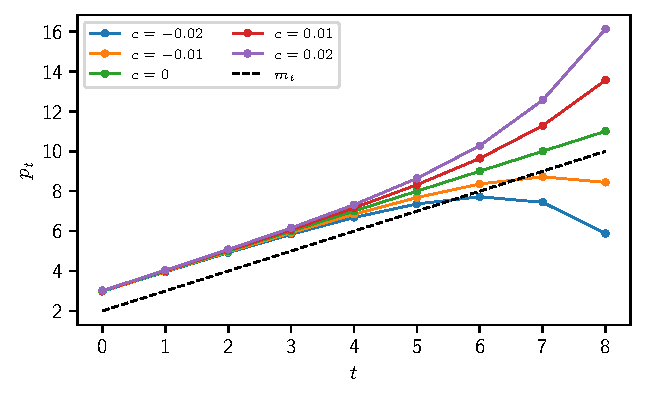
\includegraphics[width=.7\textwidth]{fig/ls02_08_cagan.pdf}
\captionof{figure}{Exercise 2.8(e): equilibrium price paths $p_t=m_t+g+c\,2^t$ for five values of
$c$ ($\alpha=\rho=1$, $m_{-2}=0$, $m_{-1}=1$).}\label{fig:cagan}
\end{center}

\textbf{Verification.} \nb{2.8}: $(w_0,w_1)$ against the brute-force forward sum truncated at 700
terms for $(\alpha,\rho)\in\{(2,.6),(1,1),(3,.9)\}$; (1) holds on every plotted path. \checkmark
\end{tcolorbox}

%------- 2.9 -------
\begin{tcolorbox}[oddbox,title={Exercise 2.9 \quad Pricing with a Stochastic Discount Factor}]
\begin{tcolorbox}[questionbox]
The $n\times1$ state vector of an economy is governed by the linear stochastic difference equation
$x_{t+1}=Ax_t+C_tw_{t+1}$ (1) where $C_t$ is a possibly time-varying matrix (known at $t$) and
$w_{t+1}$ is an $m\times1$ martingale difference sequence adapted to its own history with
$Ew_{t+1}w_{t+1}'|J_t=I$, where $J_t=[w_t\ \dots\ w_1\ x_0]$. A scalar one-period payoff $p_{t+1}$ is
given by $p_{t+1}=Px_{t+1}$ (2). The stochastic discount factor for this economy is a scalar $m_{t+1}$
that obeys $m_{t+1}=\frac{Mx_{t+1}}{Mx_t}$ (3). Finally, the price at time $t$ of the one-period
payoff is given by $q_t=f_t(x_t)$, where $f_t$ is some possibly time-varying function of the state.
That $m_{t+1}$ is a stochastic discount factor means that $E(m_{t+1}p_{t+1}|J_t)=q_t$ (4).\\[3pt]
(a) Compute $f_t(x_t)$, describing in detail how it depends on $A$ and $C_t$.\\
(b) Suppose that an econometrician has a time series data set
$X_t=[z_t\ m_{t+1}\ p_{t+1}\ q_t]$, for $t=1,\dots,T$, where $z_t$ is a strict subset of the variables
in the state $x_t$. Assume that investors in the economy see $x_t$ even though the econometrician sees
only a subset $z_t$ of $x_t$. Briefly describe a way to use these data to test implication (4).
(Possibly but perhaps not useful hint: recall the law of iterated expectations.)
\end{tcolorbox}

\textbf{Solution:}

\begin{enumerate}
\item $M$ and $P$ are $1\times n$, so $Mx_{t+1}$ and $Px_{t+1}$ are scalars and
$(Mx_{t+1})(Px_{t+1})=Mx_{t+1}x_{t+1}'P'$. Since $Mx_t$ is known at $t$,
\[
q_t=\frac{M\,E[x_{t+1}x_{t+1}'|J_t]\,P'}{Mx_t}.
\]
From (1), $E[x_{t+1}x_{t+1}'|J_t]=Ax_tx_t'A'+C_tE[w_{t+1}w_{t+1}'|J_t]C_t'=Ax_tx_t'A'+C_tC_t'$ (the
cross terms vanish because $E[w_{t+1}|J_t]=0$). Therefore
\[
\boxed{f_t(x_t)=\frac{(MAx_t)(PAx_t)+MC_tC_t'P'}{Mx_t}}
=\underbrace{E_t[m_{t+1}]\,E_t[p_{t+1}]}_{\text{``risk-neutral'' part}}+\underbrace{\Cov_t(m_{t+1},p_{t+1})}_{\text{risk adjustment}}.
\]
$A$ enters through the conditional means $MAx_t,PAx_t$; $C_t$ only through the conditional covariance
$MC_tC_t'P'/(Mx_t)$, which is the \textbf{only} source of time variation in $f_t$ beyond $x_t$ itself.
If $C_t=0$ the price is the discounted certainty equivalent. (We need $Mx_t\neq0$.)
\item Define the pricing error $e_{t+1}=m_{t+1}p_{t+1}-q_t$; (4) says $E[e_{t+1}|J_t]=0$. The
econometrician's information $\mathcal I_t=\{z_t,X_{t-1},X_{t-2},\dots\}$ is contained in $J_t$, so by
the law of iterated expectations $E[e_{t+1}|\mathcal I_t]=E\{E[e_{t+1}|J_t]|\mathcal I_t\}=0$. Hence
for any vector of instruments $h_t$ measurable with respect to $\mathcal I_t$ (e.g.\ $h_t=[1,z_t,
m_t,p_t,q_{t-1}]'$), $E[e_{t+1}h_t]=0$. All pieces of $e_{t+1}$ are in the data, even though $x_t$ is
not. Form $g_T=\frac1T\sum_te_{t+1}h_t$ and test $g_T\approx0$ with Hansen's GMM $J$-statistic
$Tg_T'\hat S^{-1}g_T\sim\chi^2(\dim h)$, $\hat S$ a HAC estimate of the long-run variance of
$e_{t+1}h_t$ (by (4), $e_{t+1}h_t$ is itself a martingale difference, so no lags are needed).
\end{enumerate}

\textbf{Verification.} \nb{2.9}: formula $-13.5407$ vs.\ Monte Carlo ($2\times10^6$ draws) $-13.5340$ at a random state. \checkmark
\end{tcolorbox}

%------- 2.29 -------
\begin{tcolorbox}[oddbox,title={Exercise 2.29 \quad Pure Prediction}]
\begin{tcolorbox}[questionbox]
Consider the Bellman equation $\mu_t=Rx_t+A'\mu_{t+1}$ (1), where $x_{t+1}=Ax_t$. Here $x_t$ is an
$n\times1$ vector, $A$ is an $n\times n$ stable matrix, and $R$ is an $n\times n$ positive definite
matrix.\\[3pt]
(a) Show that $\mu_t=R\sum_{j=0}^\infty A'^jx_{t+j}$ (2) is a solution of the forward-looking
difference equation (1).\\
(a$'$) Guess that $\mu_t=Px_t$, then verify that $P=R+A'PA$ (3).\\
(c) Please compare formula (3) for $P$ with formula (2.4.10) for the unconditional covariance matrix
of a vector governed by an autoregression.\\
(d) Please compare formula (3) with the formula (2.4.25) for $P$ that is a key step in the Howard
policy improvement algorithm.\\
(e) Can you invent a counterpart of the Howard policy improvement algorithm to compute a
time-invariant version of the Kalman filter?
\end{tcolorbox}

\textbf{Solution:}

\begin{enumerate}
\item The correct solution has $R$ \emph{inside} the sum: $\mu_t=\sum_{j=0}^\infty A'^jRx_{t+j}$.
Check:
\[
Rx_t+A'\mu_{t+1}=Rx_t+\sum_{j\ge0}A'^{j+1}Rx_{t+1+j}=Rx_t+\sum_{k\ge1}A'^kRx_{t+k}=\mu_t.\ \checkmark
\]
The sum converges because $x_{t+k}=A^kx_t$ and $\|A'^kRA^k\|\le c\,r^{2k}$ for any $r$ above the
spectral radius of $A$, which is $<1$. The printed form $R\sum_jA'^jx_{t+j}$ gives
$Rx_t+A'R\sum_jA'^jx_{t+1+j}$, which equals it only if $A'R=RA'$; see the trap box.
\item[(a$'$)] Substituting $x_{t+j}=A^jx_t$: $\mu_t=\big(\sum_{j\ge0}A'^jRA^j\big)x_t\equiv Px_t$. Then
$P-A'PA=\sum_{j\ge0}A'^jRA^j-\sum_{j\ge1}A'^jRA^j=R$, i.e.\ $\boxed{P=R+A'PA}$. Directly from (1):
$Px_t=Rx_t+A'PAx_t$ for all $x_t$ gives the same equation.
\item[(c)] (2.4.10) is $\Sigma_\infty=A\Sigma_\infty A'+CC'$, with solution $\sum_jA^jCC'A'^j$. It is
the same discrete Lyapunov equation with $A\leftrightarrow A'$ and $CC'\leftrightarrow R$: the
\textbf{dual}. $\Sigma_\infty$ accumulates past shocks forward through $A$; $P$ accumulates future
payoffs backward through $A'$.
\item[(d)] (2.4.25) is $P_0=(R+F_0'QF_0)+\big(\sqrt\beta(A-BF_0)\big)'P_0\big(\sqrt\beta(A-BF_0)\big)$:
formula (3) with $R\to R+F_0'QF_0$ and $A\to\sqrt\beta(A-BF_0)$. The policy-evaluation step of Howard's
algorithm is a pure prediction problem: the value of a fixed rule is a discounted sum of future
quadratic payoffs along the closed-loop law of motion.
\item[(e)] Yes, by duality. \emph{Evaluation:} for a fixed gain $K$ with $A-KG$ stable, the steady-state
error $e_t=x_t-\hat x_t$ obeys $e_{t+1}=(A-KG)e_t+Cw_{t+1}-Kv_t$, so its covariance solves the Lyapunov
equation
\[
\Sigma_K=(A-KG)\Sigma_K(A-KG)'+CC'+KRK'\qquad\text{(cf. (2.7.14d) with $K$ held fixed).}
\]
\emph{Improvement:} given $\Sigma_K$, choose the gain that minimises next period's error covariance
$(A-KG)\Sigma_K(A-KG)'+KRK'$; the first-order condition $-2A\Sigma_KG'+2K(G\Sigma_KG'+R)=0$ gives
$K_{\text{new}}=A\Sigma_KG'(G\Sigma_KG'+R)^{-1}$ (2.7.14b). Iterate until $K$ settles, starting from a
$K_0$ with $A-K_0G$ stable ($K_0=0$ if $A$ is stable). This mirrors (2.4.30) under the duality
$A\to A'$, $B\to G'$, $R\to CC'$, $Q\to R$, $F\to K'$, $\beta=1$.
\end{enumerate}

\textbf{Verification.} \nb{2.29}: $P$ from a Lyapunov solver against $\sum_{j<400}A'^jRA^j$; residual of
(1) is $4\times10^{-14}$ with the $A'^jR$ order and $9.4$ with the printed order; the Howard-Kalman
iteration converges in 6 steps to the Riccati fixed point for two systems. \checkmark
\end{tcolorbox}

\begin{tcolorbox}[trapbox]
Formula (2) as printed, $\mu_t=R\sum_jA'^jx_{t+j}$, is not a solution of (1) unless $R$ commutes with
$A'$ (e.g.\ $R=rI$ or scalar $x$). The weighting matrix must sit between the powers of $A'$ and the
future state: $\mu_t=\sum_jA'^jRx_{t+j}$. The notebook shows the printed version failing (1) for a
random $3\times3$ example.
\end{tcolorbox}

%======================================================================
\subsection{Spectra}
%======================================================================

%------- 2.7 -------
\begin{tcolorbox}[oddbox,title={Exercise 2.7 \quad Simulations, Impulse Responses and Spectra}]
\begin{tcolorbox}[questionbox]
Get the Matlab programs \texttt{bigshow3.m} and \texttt{freq.m} from
\texttt{<www.tomsargent.com/source\_code/mitbook.zip>}. Use \texttt{bigshow3} to compute and display
a simulation of length 80, an impulse response function, and a spectrum for each of the following
scalar stochastic processes $y_t$. In each of the following, $w_t$ is a scalar martingale difference
sequence adapted to its own history and the initial values of lagged $y$'s.\\[3pt]
a.\ $y_t=w_t$.\quad b.\ $y_t=(1+.5L)w_t$.\quad c.\ $y_t=(1+.5L+.4L^2)w_t$.\quad
d.\ $(1-.999L)y_t=(1-.4L)w_t$.\quad e.\ $(1-.8L)y_t=(1+.5L+.4L^2)w_t$.\quad
f.\ $(1+.8L)y_t=w_t$.\quad g.\ $y_t=(1-.6L)w_t$.\\
Study the output and look for patterns. When you are done, you will be well on your way to knowing
how to read spectral densities.
\end{tcolorbox}

\textbf{Solution:}

Write each process as $a(L)y_t=b(L)w_t$ with $Ew_t^2=1$. The impulse response is
$h(L)=b(L)/a(L)$, and by (2.11.2) with $y=Gx$ the spectrum is
\[
S_y(\omega)=h(e^{-i\omega})h(e^{i\omega})=\frac{|b(e^{-i\omega})|^2}{|a(e^{-i\omega})|^2},
\qquad S_y(0)=\frac{b(1)^2}{a(1)^2},\quad S_y(\pi)=\frac{b(-1)^2}{a(-1)^2}.
\]
The Python counterpart of \texttt{bigshow3} (\nb{2.7}) produces Figure~\ref{fig:bigshow}.

\begin{center}\small
\begin{tabular}{@{}lcccl@{}}
\toprule
 & $\Var(y)=\sum h_j^2$ & $S(0)$ & $S(\pi)$ & shape\\
\midrule
a & 1 & 1 & 1 & flat\\
b & 1.25 & 2.25 & .25 & falls from $0$ to $\pi$\\
c & 1.41 & 3.61 & .81 & falls, dip near $\omega\approx2$\\
d & 180.49 & 360000 & .49 & enormous spike at $\omega=0$\\
e & 8.45 & 90.25 & .25 & low-frequency power, dip near $\omega\approx2.1$\\
f & 2.78 & .31 & 25 & rises to a peak at $\pi$\\
g & 1.36 & .16 & 2.56 & rises from $0$ to $\pi$\\
\bottomrule
\end{tabular}
\end{center}

\textbf{Patterns.}
\begin{itemize}
\item \emph{White noise (a)} has a flat spectrum: every frequency contributes equally, the impulse
response is a single spike, and the path has no visible persistence.
\item \emph{Positive MA coefficients (b, c)} smooth the noise: neighbouring $y$'s share shocks, the
impulse response is cut off after $q$ lags, and power moves to low frequencies. A zero of $b(z)$ near
the unit circle creates a trough in $S_y$; in (c) the zeros of $1+.5z+.4z^2$ have modulus
$1/\sqrt{.4}=1.58$ and angle $\approx2$, hence the dip there.
\item \emph{Near unit root (d).} $(1-.999L)^{-1}$ makes the impulse response almost flat at
$.999-.4=.599$ after lag 0, and $S_y(0)=(.6/.001)^2=360000$: nearly all variance sits at very low
frequency. This is Granger's ``typical spectral shape'' in its extreme form; the simulation wanders.
It is the Muth process of Figure 2.11.4 and section 2.10.1, where most of a shock is permanent.
\item \emph{Mixed (e).} The AR(1) factor adds low-frequency power and the MA factor keeps the dip of
(c); the impulse response is hump-shaped (peaks at lag 2).
\item \emph{Negative AR root (f).} $(1+.8L)^{-1}$ gives an impulse response alternating in sign,
$(-.8)^j$, so the path zig-zags and power piles up at $\omega=\pi$ (period 2).
\item \emph{Negative MA coefficient (g).} Opposite of (b): it is a partial difference, so it removes
low-frequency power, $S(0)=(1-.6)^2=.16$.
\end{itemize}
Rule of thumb: smooth, persistent paths and slowly decaying same-sign impulse responses mean power at
low frequencies; choppy paths and sign-alternating responses mean power near $\pi$; a spectral
peak inside $(0,\pi)$ means a pseudo-cycle (Exercise 2.15).

\textbf{Verification.} \nb{2.7}: for each process, $\frac1{2\pi}\int_{-\pi}^\pi S_y$ equals
$\sum_jh_j^2$ to relative error $10^{-4}$. \checkmark
\end{tcolorbox}

\begin{center}
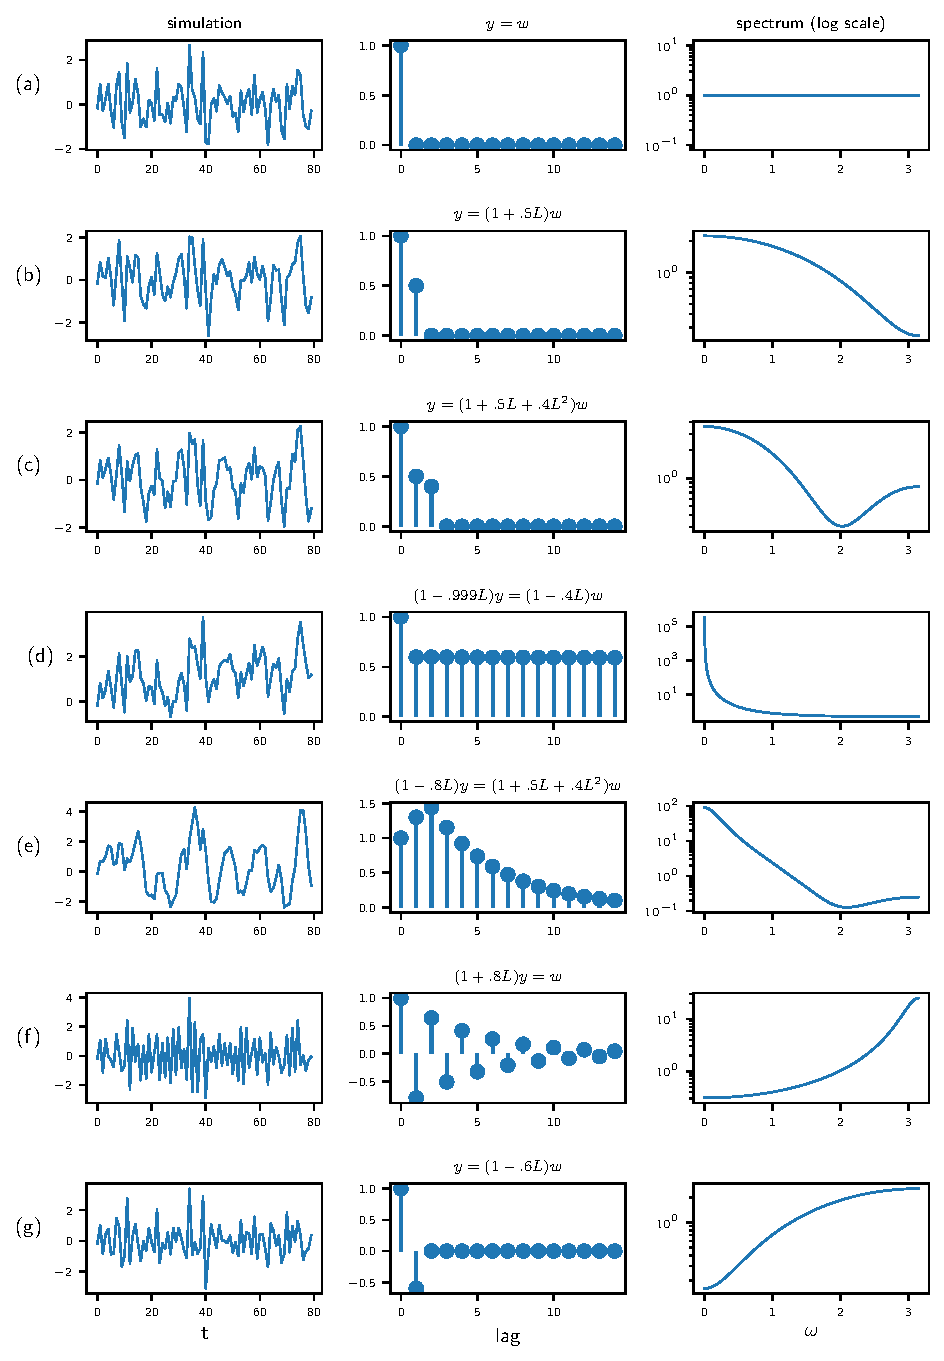
\includegraphics[height=.86\textheight,keepaspectratio]{fig/ls02_07_bigshow.pdf}
\captionof{figure}{Exercise 2.7: simulation (length 80, common shocks), impulse response and spectrum
(log scale) for processes a--g.}\label{fig:bigshow}
\end{center}

%------- 2.15 -------
\begin{tcolorbox}[oddbox,title={Exercise 2.15 \quad The Slutsky Effect}]
\begin{tcolorbox}[questionbox]
Suppose that a scalar is related to a scalar white noise $w_t$ with variance 1 by $y_t=h(L)w_t$
where $h(L)=\sum_{j=0}^\infty L^jh_j$ and $\sum_{j=0}^\infty h_j^2<+\infty$. Then a special case of
formula (2.11.2) coupled with the observer equation $y_t=Gx_t$ implies that the spectrum of $y$ is
given by $S_y(\omega)=h(\exp(-i\omega))h(\exp(i\omega))=|h(\exp(-i\omega))|^2$ where
$h(\exp(-i\omega))=\sum_{j=0}^\infty h_j\exp(-i\omega j)$. In a famous paper, Slutsky investigated the
consequences of applying the following filter to white noise: $h(L)=(1+L)^n(1-L)^m$ (i.e., the
convolution of $n$ two-period moving averages with $m$ difference operators). Compute and plot the
spectrum of $y$ for $\omega\in[-\pi,\pi]$ for the following choices of $m,n$:\\[3pt]
(a) $m=10,n=10$.\quad (b) $m=10,n=40$.\quad (c) $m=40,n=10$.\quad (d) $m=120,n=30$.\\
(e) Comment on these results.
\textit{Hint:} Notice that $h(\exp(-i\omega))=(1+\exp(-i\omega))^n(1-\exp(-i\omega))^m$.
\end{tcolorbox}

\textbf{Solution:}

\emph{Closed form.} $|1+e^{-i\omega}|^2=(1+\cos\omega)^2+\sin^2\omega=2+2\cos\omega=4\cos^2\frac\omega2$ and
$|1-e^{-i\omega}|^2=2-2\cos\omega=4\sin^2\frac\omega2$. Hence
\[
S_y(\omega)=(2+2\cos\omega)^n(2-2\cos\omega)^m=4^{n+m}\cos^{2n}\!\tfrac\omega2\,\sin^{2m}\!\tfrac\omega2,
\]
symmetric in $\omega$, with $S_y(0)=0$ (for $m\ge1$) and $S_y(\pm\pi)=0$ (for $n\ge1$).

\emph{Peak.} $\frac{d}{d\omega}\log S_y=-n\tan\frac\omega2+m\cot\frac\omega2=0\Rightarrow
\tan^2\frac{\omega}{2}=\frac mn$, so
\[
\boxed{\omega^*=2\arctan\sqrt{m/n}}.
\]
\emph{Sharpness.} $\frac{d^2}{d\omega^2}\log S_y=-\frac n2\sec^2\frac\omega2-\frac m2\csc^2\frac\omega2$;
at $\omega^*$, $\sec^2=\frac{n+m}{n}$ and $\csc^2=\frac{n+m}{m}$, so the curvature is $-(n+m)$ and
$S_y\approx S_y(\omega^*)e^{-(n+m)(\omega-\omega^*)^2/2}$: a Gaussian bump of width $1/\sqrt{n+m}$, with
half-power width $2\sqrt{2\ln2/(n+m)}$.

\begin{center}\small
\begin{tabular}{@{}lcccccc@{}}
\toprule
 & $m$ & $n$ & $\omega^*$ & period & half-power width (num./formula) & $\log_{10}S(\omega^*)$\\
\midrule
a & 10 & 10 & $\pi/2=1.5708$ & 4.00 & .5235 / .5265 & 6.02\\
b & 10 & 40 & .9273 & 6.78 & .3319 / .3330 & 19.24\\
c & 40 & 10 & 2.2143 & 2.84 & .3319 / .3330 & 19.24\\
d & 120 & 30 & 2.2143 & 2.84 & .1920 / .1923 & 57.71\\
\bottomrule
\end{tabular}
\end{center}

\begin{enumerate}[start=5]
\item \emph{Comment.} Summing ($n$) is a low-pass filter; differencing ($m$) is high-pass. Composing them
gives a band-pass filter whose output has a single sharp spectral peak inside $(0,\pi)$, i.e.\ a
nearly periodic ``cycle'' of period $2\pi/\omega^*$, although the input is serially uncorrelated.
This is the \textbf{Slutsky effect}: mechanical smoothing and differencing of pure noise can
manufacture regular-looking business cycles. The ratio $m/n$ locates the cycle (more differencing, a
shorter period: (b) vs.\ (c)); the total $m+n$ sets how regular it is (same $\omega^*$ in (c) and
(d), but (d) is much narrower). The levels are astronomically large ($10^{57}$ in (d)), so the plot
normalises each spectrum by its maximum (Figure~\ref{fig:slutsky}).
\end{enumerate}

\textbf{Verification.} \nb{2.15}: numerical argmax on a grid of $200{,}001$ points matches
$\omega^*$ within $10^{-4}$. \checkmark
\end{tcolorbox}

\begin{center}
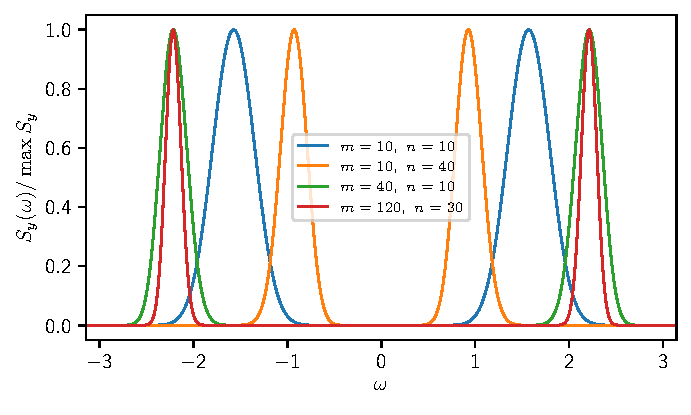
\includegraphics[width=.72\textwidth]{fig/ls02_15_slutsky.pdf}
\captionof{figure}{Exercise 2.15: normalised spectra $S_y(\omega)/\max S_y$ of Slutsky's filter.}\label{fig:slutsky}
\end{center}

%======================================================================
\subsection{The Kalman Filter, Innovations and VARs}
%======================================================================

%------- 2.19 -------
\begin{tcolorbox}[oddbox,title={Exercise 2.19 \quad IQ}]
\begin{tcolorbox}[questionbox]
An infinitely lived person's `true intelligence' $\theta\sim\mathcal N(100,100)$, i.e., mean 100,
variance 100. For each date $t\ge0$, the person takes a `test' with the outcome being a univariate
random variable $y_t=\theta+v_t$, where $v_t$ is an iid process with distribution $\mathcal N(0,100)$.
The person's initial IQ is $IQ_0=100$ and at date $t\ge1$ before the date $t$ test is taken it is
$\text{IQ}_t=E\theta|y^{t-1}$, where $y^{t-1}$ is the history of test scores from date 0 until date
$t-1$.\\[3pt]
(a) Give a recursive formula for $\text{IQ}_t$ and for $E(\text{IQ}_t-\theta)^2$.\\
(b) Use Matlab to simulate 10 draws of $\theta$ and associated paths of $y_t,\text{IQ}_t$ for
$t=0,\dots,50$.\\
(c) Prove that $\lim_{t\to\infty}E(\text{IQ}_t-\theta)^2=0$.
\end{tcolorbox}

\textbf{Solution:}

This is the Kalman filter (2.7.14) with $x_t=\theta$, $A=1$, $C=0$, $G=1$, $R=100$, $\hat x_0=100$,
$\Sigma_0=100$, and $\hat x_t=\text{IQ}_t$ (Jovanovic's application, section 2.10.2).
\begin{enumerate}
\item From (2.7.14b,c,d) with $A=1,C=0$:
\[
K_t=\frac{\Sigma_t}{\Sigma_t+100},\qquad \boxed{\text{IQ}_{t+1}=\text{IQ}_t+K_t(y_t-\text{IQ}_t)},
\]
\[
\boxed{\Sigma_{t+1}=(1-K_t)^2\Sigma_t+K_t^2\,100=\frac{100\,\Sigma_t}{\Sigma_t+100}},
\]
with $\Sigma_t=E(\text{IQ}_t-\theta)^2$. \emph{Closed forms.} Inverting, $\frac1{\Sigma_{t+1}}=
\frac1{\Sigma_t}+\frac1{100}$ (2.10.9), so $\frac{1}{\Sigma_t}=\frac{t+1}{100}$, i.e.\
$\Sigma_t=\frac{100}{t+1}$ and $K_t=\frac{1}{t+2}$. Then $(t+2)\text{IQ}_{t+1}=(t+1)\text{IQ}_t+y_t$;
telescoping from $\text{IQ}_0=100$:
\[
\text{IQ}_t=\frac{100+\sum_{s=0}^{t-1}y_s}{t+1}.
\]
Because the prior variance equals the noise variance, the prior counts as exactly one extra test
with score 100.
\item Figure~\ref{fig:iq}: ten draws of $\theta$ and the implied IQ paths.
\item $E(\text{IQ}_t-\theta)^2=\Sigma_t=\frac{100}{t+1}\to0$. $\blacksquare$ (At $t=50$,
$\Sigma_{50}=1.96$.) Precision grows linearly in the number of tests.
\end{enumerate}

\textbf{Verification.} \nb{2.19}: the recursion reproduces both closed forms on every path. \checkmark
\end{tcolorbox}

\begin{center}
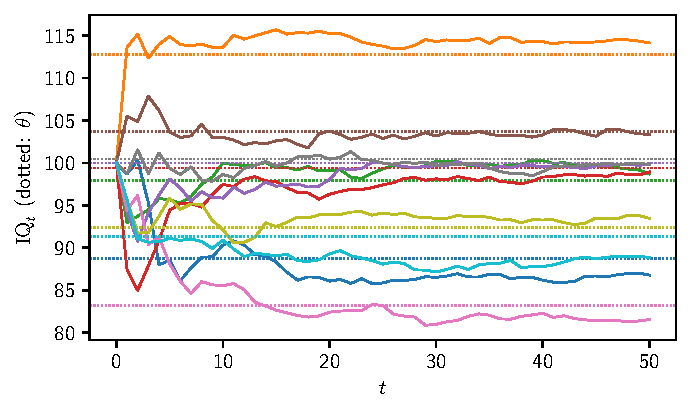
\includegraphics[width=.7\textwidth]{fig/ls02_19_iq.pdf}
\captionof{figure}{Exercise 2.19: $\text{IQ}_t$ for ten draws of $\theta$ (dotted lines).}\label{fig:iq}
\end{center}

%------- 2.26 -------
\begin{tcolorbox}[evenbox,title={Exercise 2.26 \quad Math and Verbal IQ's}]
\begin{tcolorbox}[questionbox]
An infinitely lived person's `true intelligence' $\theta$ has two components, math ability
$\theta_1$ and verbal ability $\theta_2$, where
$\theta\sim\mathcal N\left(\begin{bmatrix}100\\100\end{bmatrix},\begin{bmatrix}100&0\\0&100\end{bmatrix}\right)$.
For each date $t\ge0$, the person takes a single `test' with the outcome being a univariate random
variable $y_t=G_t\theta+v_t$, where $v_t$ is an iid process with distribution $\mathcal N(0,50)$ and
$G_t=[.9\ .1]$ for $t=0,2,4,\dots$ and $G_t=[.01\ .99]$ for $t=1,3,5,\dots$. Here the person takes a
math test at $t$ even and a verbal test at $t$ odd (but you have to know how to read English to
survive the math test, and you have to know how to tell time in order to plan your time allocation
well for the verbal test). The person's initial IQ vector is $IQ_0=\begin{bmatrix}100\\100\end{bmatrix}$
and at date $t\ge1$ before the date $t$ test is taken it is $\text{IQ}_t=E\theta|y^{t-1}$, where
$y^{t-1}$ is the history of test scores from date 0 until date $t-1$.\\[3pt]
(a) Give a recursive formula for $\text{IQ}_t$ and for $E(\text{IQ}_t-\theta)(\text{IQ}_t-\theta)'$.\\
(b) Use Matlab to simulate 10 draws of $\theta$ and associated paths of $y_t,\text{IQ}_t$ for
$t=0,\dots,50$.\\
(c) Show computationally or analytically that
$\lim_{t\to+\infty}E(\text{IQ}_t-\theta)(\text{IQ}_t-\theta)'=\begin{bmatrix}0&0\\0&0\end{bmatrix}$.
\end{tcolorbox}

\textbf{Solution:}

Kalman filter with $A=I_2$, $C=0$, $R=50$ and a \textbf{time-varying} $G_t$; $\Sigma_0=100I$.
\begin{enumerate}
\item With $G_t\Sigma_tG_t'+50$ a scalar,
\[
K_t=\frac{\Sigma_tG_t'}{G_t\Sigma_tG_t'+50},\qquad
\text{IQ}_{t+1}=\text{IQ}_t+K_t\,(y_t-G_t\text{IQ}_t),
\]
\[
\Sigma_{t+1}=\Sigma_t-\frac{\Sigma_tG_t'G_t\Sigma_t}{G_t\Sigma_tG_t'+50},
\]
and $E(\text{IQ}_t-\theta)(\text{IQ}_t-\theta)'=\Sigma_t$. (This is (2.7.14) with $A=I$, $C=0$: the
$(A-KG)\Sigma(A-KG)'+KRK'$ form simplifies to the one shown.)
\item Figure~\ref{fig:iq2}.
\item By the matrix inversion lemma the covariance update is, in precision form,
\[
\Sigma_{t+1}^{-1}=\Sigma_t^{-1}+\frac{G_t'G_t}{50}\quad\Rightarrow\quad
\Sigma_t^{-1}=\frac{I}{100}+\frac1{50}\sum_{s=0}^{t-1}G_s'G_s .
\]
Each pair of periods adds
\[
M=\frac{1}{50}\left(\begin{bmatrix}.81&.09\\.09&.01\end{bmatrix}+\begin{bmatrix}.0001&.0099\\.0099&.9801\end{bmatrix}\right)
=\begin{bmatrix}.016202&.001998\\.001998&.019802\end{bmatrix},
\]
positive definite (eigenvalues $.015313$ and $.020691$). Hence
$\lambda_{\min}(\Sigma_t^{-1})\ge\lfloor t/2\rfloor\,(.015313)\to\infty$ and
$\|\Sigma_t\|=1/\lambda_{\min}(\Sigma_t^{-1})\to0$. $\blacksquare$ Numbers:
$\Sigma_{50}=\begin{bmatrix}2.438&-.241\\-.241&2.004\end{bmatrix}$,
$\Sigma_{5000}=\begin{bmatrix}.0250&-.0025\\-.0025&.0205\end{bmatrix}$.
\end{enumerate}
\emph{Reading.} Each test alone is rank-one information, so repeating only the math test would leave
the direction orthogonal to $[.9,.1]$ unlearned: $\Sigma_t$ would not vanish. It is the
\textbf{alternation} of two linearly independent tests that identifies both abilities. The negative
off-diagonal arises because each score loads positively on both abilities: a high math score is
partly attributed to verbal ability, so the two estimation errors move in opposite directions.

\textbf{Verification.} \nb{2.26}: the recursion reproduces the precision form at $t=50$. \checkmark
\end{tcolorbox}

\begin{center}
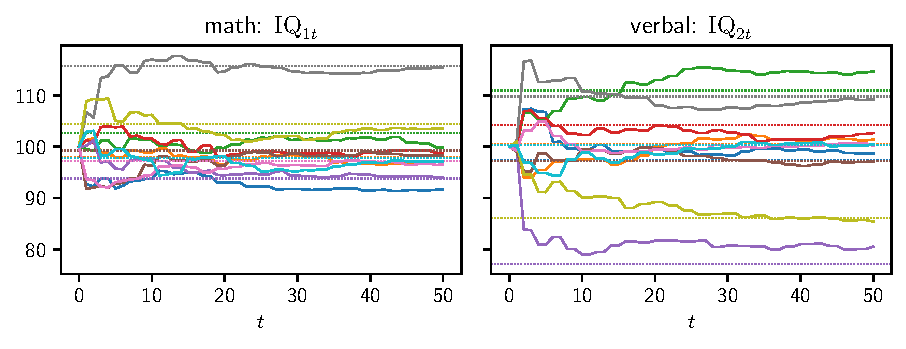
\includegraphics[width=\textwidth]{fig/ls02_26_iq2.pdf}
\captionof{figure}{Exercise 2.26: math and verbal IQ for ten draws of $\theta$ (dotted: true values).}\label{fig:iq2}
\end{center}

%------- 2.20 -------
\begin{tcolorbox}[evenbox,title={Exercise 2.20 \quad Random Walk Seen Through Two Signals}]
\begin{tcolorbox}[questionbox]
A scalar process $x_t$ follows the process $x_{t+1}=x_t+w_{t+1}$ where $w$ is an iid $\mathcal N(0,1)$
scalar process and $x_0\sim\mathcal N(\hat x_0,\Sigma_0)$. Each period, an observer receives two signals
in the form of a $2\times1$ vector $y_t$ that obeys $y_t=\begin{bmatrix}1\\1\end{bmatrix}x_t+v_t$ where
the $2\times1$ process $v_t$ is iid with distribution $v_t\sim\mathcal N(0,R)$ where
$R=\begin{bmatrix}1&0\\0&1\end{bmatrix}$.\\[3pt]
(a) Suppose that $\Sigma_0=1.36602540378444$. For $t\ge0$, find formulas for $E[x_t|y^{t-1}]$, where
$y^{t-1}$ is the history of $y_s$ for $s$ from 0 to $t-1$.\\
(b) Verify numerically that the matrix $A-KG$ in formula (2.9.3) is stable.\\
(c) Find an infinite-order vector autoregression for $y_t$.
\end{tcolorbox}

\textbf{Solution:}

$A=1$, $C=1$, $G=\mathbf 1=[1,1]'$, $R=I_2$.
\begin{enumerate}
\item \emph{Riccati map.} By Sherman--Morrison, $(\Sigma\mathbf 1\mathbf 1'+I)^{-1}=I-\frac{\Sigma}{1+2\Sigma}\mathbf 1\mathbf 1'$,
so $\mathbf 1'(\Sigma\mathbf 1\mathbf 1'+I)^{-1}\mathbf 1=2-\frac{4\Sigma}{1+2\Sigma}=\frac{2}{1+2\Sigma}$.
(2.7.15) becomes
\[
\Sigma_{t+1}=\Sigma_t+1-\frac{2\Sigma_t^2}{1+2\Sigma_t}=\frac{3\Sigma_t+1}{2\Sigma_t+1}.
\]
Fixed point: $\Sigma(2\Sigma+1)=3\Sigma+1\Rightarrow2\Sigma^2-2\Sigma-1=0\Rightarrow
\Sigma=\frac{1+\sqrt3}{2}=1.36602540378444$: the given $\Sigma_0$ \textbf{is} the fixed point, so
$\Sigma_t=\Sigma_0$ and the filter is time invariant from $t=0$.
\emph{Gain.} $K=\Sigma\mathbf 1'(\Sigma\mathbf 1\mathbf 1'+I)^{-1}=\frac{\Sigma}{1+2\Sigma}\mathbf 1'$; with
$1+2\Sigma=2+\sqrt3$, $\frac{\Sigma}{1+2\Sigma}=\frac{(1+\sqrt3)(2-\sqrt3)}{2}=\frac{\sqrt3-1}{2}\equiv k=.366025$.
Hence, with $1-2k=2-\sqrt3=.267949$,
\[
\begin{aligned}
&\boxed{\hat x_{t+1}=(2-\sqrt3)\,\hat x_t+k\,(y_{1t}+y_{2t})},\\
&E[x_t|y^{t-1}]=\hat x_t=(2-\sqrt3)^t\hat x_0+k\sum_{j=0}^{t-1}(2-\sqrt3)^j\,(y_{1,t-1-j}+y_{2,t-1-j}).
\end{aligned}
\]
The two signals are symmetric, so only their sum matters.
\item $A-KG=1-2k=2-\sqrt3=.2679$, inside the unit circle. \checkmark
\item From (2.9.3), $y_t=G\sum_{j\ge0}(A-KG)^jKy_{t-j-1}+a_t$:
\[
\boxed{y_t=\begin{bmatrix}1\\1\end{bmatrix}k\sum_{j=0}^\infty(2-\sqrt3)^j\,[1\ \ 1]\,y_{t-1-j}+a_t},
\]
\[
Ea_ta_t'=\Sigma\mathbf 1\mathbf 1'+I=\begin{bmatrix}2.366025&1.366025\\1.366025&2.366025\end{bmatrix}.
\]
Each equation has the same coefficients, $A_j=k(2-\sqrt3)^{j-1}\mathbf 1\mathbf 1'$, $j\ge1$.
\end{enumerate}

\textbf{Verification.} \nb{2.20}: Riccati iteration converges to $(1+\sqrt3)/2$; one step from
$\Sigma_0$ leaves it unchanged; in a $200{,}000$-period simulation the innovations have sample
covariance within $.05$ of $G\Sigma G'+R$ and lag-1 autocovariances below $.01$. \checkmark
\end{tcolorbox}

%------- 2.21 -------
\begin{tcolorbox}[oddbox,title={Exercise 2.21 \quad Impulse Response for a VAR}]
\begin{tcolorbox}[questionbox]
Find the impulse response function for the state space representation (2.9.1) associated with a
vector autoregression.
\end{tcolorbox}

\textbf{Solution:}

(2.9.1): $\hat x_{t+1}=A\hat x_t+Ka_t$, $y_t=G\hat x_t+a_t$, $Ea_ta_t'=G\Sigma G'+R\equiv\Omega$. Iterating
the state equation backward, $\hat x_t=\sum_{j\ge1}A^{j-1}Ka_{t-j}$ (plus $A^t\hat x_0$ from a finite
start), so
\[
y_t=a_t+\sum_{j=1}^\infty GA^{j-1}K\,a_{t-j}.
\]
\[
\boxed{\frac{\partial y_{t+j}}{\partial a_t'}=\Psi_j=\begin{cases}I_m,&j=0\\ GA^{j-1}K,&j\ge1\end{cases}}
\]
Equivalently, the VAR $y_t=\sum_{j\ge1}\Phi_jy_{t-j}+a_t$ with $\Phi_j=G(A-KG)^{j-1}K$ (2.9.3) inverts to
the same $\Psi$ via $\Psi_0=I$, $\Psi_j=\sum_{k=1}^j\Phi_k\Psi_{j-k}$: the two recursions describe the
same linear system ($\hat x_{t+1}=(A-KG)\hat x_t+Ky_t$ is (2.9.1a) with $a_t=y_t-G\hat x_t$
substituted). Because the $a_t$'s are contemporaneously correlated, the usual practice is to report
responses to orthonormalised shocks $\Psi_jL$, with $\Omega=LL'$ (Cholesky); that step imposes a
recursive ordering and is not implied by (2.9.1). When $A$ has a unit eigenvalue (Exercise 2.20),
$\Psi_j$ need not die out: there $\Psi_j=k\mathbf 1\mathbf 1'$ for all $j\ge1$ (a shock to the
random-walk estimate is permanent).

\textbf{Verification.} \nb{2.21}: $GA^{j-1}K$ equals the VAR inversion for $j<15$ on the system of
Exercise 2.20. \checkmark
\end{tcolorbox}

%------- 2.22 -------
\begin{tcolorbox}[evenbox,title={Exercise 2.22 \quad Kalman Filter with Cross-Products}]
\begin{tcolorbox}[questionbox]
Consider the state space system $x_{t+1}=Ax_t+Cw_{t+1}$, $y_{t+1}=Gx_t+Dw_{t+1}$ where $x_t$ is an
$n\times1$ state vector $w_{t+1}$ is an $m\times1$ iid process with distribution $\mathcal N(0,I)$, $y_t$
is an $m\times1$ vector of observed variables, and $x_0\sim\mathcal N(\hat x_0,\Sigma_0)$. For $t\ge1$,
$\hat x_t=E[x_t|y^t]$ where $y^t=[y_t,\dots,y_1]$ and $\Sigma_t=E(x_t-\hat x_t)(x_t-\hat x_t)'$.\\[3pt]
(a) Show how to select $w_{t+1},C$, and $D$ so that $Cw_{t+1}$ and $Dw_{t+1}$ are mutually uncorrelated
processes. Also give an example in which $Cw_{t+1}$ and $Dw_{t+1}$ are correlated.\\
(b) Construct a recursive representation for $\hat x_t$ of the form
$\hat x_{t+1}=A\hat x_t+K_ta_{t+1}$, $y_{t+1}=G\hat x_t+a_{t+1}$ where $a_{t+1}=y_{t+1}-E[y_{t+1}|y^t]$ for
$t\ge0$ and verify that
$K_t=(CD'+A\Sigma_tG')(DD'+G\Sigma_tG')^{-1}$,
$\Sigma_{t+1}=(A-K_tG)\Sigma_t(A-K_tG)'+(C-K_tD)(C-K_tD)'$ and $Ea_{t+1}a_{t+1}'=G\Sigma_tG'+DD'$.
\textit{Hint:} apply the population regression formula.
\end{tcolorbox}

\textbf{Solution:}

\begin{enumerate}
\item $E(Cw_{t+1})(Dw_{t+1})'=CD'$, so the two are uncorrelated iff $CD'=0$. Partition
$w_{t+1}=[w^x_{t+1};\,w^y_{t+1}]$ into independent blocks and set $C=[C_1\ \ 0]$, $D=[0\ \ D_2]$: then
$CD'=C_1\cdot0+0\cdot D_2'=0$ ($w$ then has as many entries as the two blocks together). This
recovers the standard system (2.7.1)--(2.7.2) with $R=D_2D_2'$, up to timing.
\emph{Correlated example:} $n=m=1$, $C=D=1$: $x_{t+1}=ax_t+w_{t+1}$, $y_{t+1}=gx_t+w_{t+1}$, so
$CD'=1$: the same shock moves the state and the signal. More generally any $C,D$ with $CD'\neq0$.
\item Let $e_t=x_t-\hat x_t$; recall $E[e_t\,|\,y^t]=0$ and $w_{t+1}\perp(x_t,y^t)$.
\emph{Step 1 (one-step predictions).} $E[x_{t+1}|y^t]=A\hat x_t$ and $E[y_{t+1}|y^t]=G\hat x_t$, so
\[
a_{t+1}=y_{t+1}-G\hat x_t=Ge_t+Dw_{t+1},\qquad x_{t+1}-A\hat x_t=Ae_t+Cw_{t+1}.
\]
\emph{Step 2 (update).} $y^{t+1}$ and $(y^t,a_{t+1})$ span the same space and $a_{t+1}\perp y^t$, so
(with normality) $\hat x_{t+1}=E[x_{t+1}|y^t]+K_ta_{t+1}=A\hat x_t+K_ta_{t+1}$, where $K_t$ is the
population regression coefficient of $x_{t+1}-A\hat x_t$ on $a_{t+1}$. Together with Step 1 this gives
the two-equation representation.
\emph{Step 3 (moments).} Using $Ee_tw_{t+1}'=0$ and $Ew_{t+1}w_{t+1}'=I$:
\[
E(Ae_t+Cw_{t+1})(Ge_t+Dw_{t+1})'=A\Sigma_tG'+CD',\qquad
\boxed{Ea_{t+1}a_{t+1}'=G\Sigma_tG'+DD'},
\]
\[
\boxed{K_t=(CD'+A\Sigma_tG')(DD'+G\Sigma_tG')^{-1}}.
\]
\emph{Step 4 (error covariance).} $e_{t+1}=x_{t+1}-\hat x_{t+1}=Ae_t+Cw_{t+1}-K_t(Ge_t+Dw_{t+1})
=(A-K_tG)e_t+(C-K_tD)w_{t+1}$, whose two terms are uncorrelated, so
\[
\boxed{\Sigma_{t+1}=(A-K_tG)\Sigma_t(A-K_tG)'+(C-K_tD)(C-K_tD)'}.
\]
\emph{Consistency.} $Ee_{t+1}a_{t+1}'=(A-K_tG)\Sigma_tG'+(C-K_tD)D'=A\Sigma_tG'+CD'-K_t(G\Sigma_tG'+DD')=0$
by the formula for $K_t$: the new error is orthogonal to the innovation, as a regression residual
must be. With $CD'=0$ and $DD'=R$ the formulas collapse to (2.7.14).
\end{enumerate}

\textbf{Verification.} \nb{2.22}: for a random $2\times2$ system with $CD'\neq0$, $\Sigma_6$ and $\hat x_6$
from the recursion equal the brute-force conditional moments of $x_6$ given $(y_1,\dots,y_6)$ computed
from the joint Gaussian covariance. \checkmark
\end{tcolorbox}

%------- 2.24 -------
\begin{tcolorbox}[evenbox,title={Exercise 2.24 \quad Stationarity}]
\begin{tcolorbox}[questionbox]
A pair of scalar stochastic processes $(z_t,y_t)$ evolves according to the state system for $t\ge0$:
$z_{t+1}=.9z_t+w_{t+1}$, $y_t=z_t+v_t$ where $w_{t+1}$ and $v_t$ are mutually uncorrelated scalar
Gaussian random variables with means of 0 and variances of 1. Furthermore, $Ew_{t+1}v_s=0$ for all
$t,s$ pairs. In addition, $z_0\sim\mathcal N(\hat z_0,\Sigma_0)$.\\[3pt]
(a) Is $\{z_t\}$ Markov? Explain.\quad (b) Is $\{y_t\}$ Markov? Explain.\\
(c) Define what it would mean for the scalar process $\{z_t\}$ to be \textit{covariance stationary}.\\
(d) Find values of $(\hat z_0,\Sigma_0)$ that make the process for $\{z_t\}$ covariance stationary.\\
(e) Assume that $y_t$ is observable, but that $z_t$ is not. Define what it would mean for the scalar
process $y_t$ to be \textit{covariance stationary}.\\
(f) Describe in as much detail as you can how to represent the distribution of $y_t$ conditional on
the infinite history $y^{t-1}$ in the form $y_t\sim\mathcal N(E[y_t|y^{t-1}],\Omega_t)$.
\end{tcolorbox}

\textbf{Solution:}

\begin{enumerate}
\item Yes. $z_{t+1}|z^t\sim\mathcal N(.9z_t,1)$ because $w_{t+1}$ is independent of $z^t$: the
conditional distribution depends on the past only through $z_t$.
\item No. $y_t$ is a noisy reading of $z_t$, and past $y$'s all carry information about $z_t$ beyond
$y_t$. Formally $(1-.9L)y_t=w_t+v_t-.9v_{t-1}$ is an ARMA(1,1), and (part f)
$E[y_{t+1}|y^t]=.537667\sum_{j\ge0}(.362333)^jy_{t-j}$ puts weight on every lag, so $y$ is not Markov
of any finite order.
\item $Ez_t=\mu$ for all $t$, and $E(z_t-\mu)(z_{t-j}-\mu)=C_z(j)$ depends only on $j$, not on $t$.
\item $Ez_t=.9^t\hat z_0$ is constant iff $\hat z_0=0$. $\Var z_{t+1}=.81\Var z_t+1$ is constant iff
$\Sigma_0=\frac1{1-.81}=5.263158$. So $\boxed{(\hat z_0,\Sigma_0)=(0,\ 1/.19)}$; then
$C_z(j)=.9^j/.19$.
\item Same definition for $y$: $Ey_t=\mu_y$ for all $t$, and $E(y_t-\mu_y)(y_{t-j}-\mu_y)=C_y(j)$
depends only on $j$. Under (d), $C_y(0)=\frac{1}{.19}+1$ and $C_y(j)=\frac{.9^j}{.19}$ for $j\ge1$;
covariance stationarity of $y$ is a statement about observables only.
\item Run the time-invariant Kalman filter (section 2.9), which conditions on the semi-infinite past:
$A=.9$, $C=1$, $G=1$, $R=1$. The Riccati equation $\Sigma=.81\Sigma+1-\frac{.81\Sigma^2}{\Sigma+1}$,
multiplied through by $\Sigma+1$, becomes $\Sigma^2+\Sigma=.81\Sigma^2+.81\Sigma+\Sigma+1-.81\Sigma^2$,
i.e.
\[
\Sigma^2-.81\Sigma-1=0\Rightarrow\Sigma=\frac{.81+\sqrt{.6561+4}}{2}=\frac{.81+2.157800}{2}=1.483900.
\]
Then $K=\frac{.9\Sigma}{\Sigma+1}=\frac{1.335510}{2.483900}=.537667$, $A-KG=.362333$, and
\[
\boxed{\begin{gathered}y_t\,|\,y^{t-1}\sim\mathcal N\big(\hat z_t,\ \Omega\big),\qquad \Omega=\Sigma+1=2.483900,\\
\hat z_t=.537667\sum_{j=0}^\infty(.362333)^jy_{t-1-j}\end{gathered}}
\]
recursively $\hat z_{t+1}=.9\hat z_t+K(y_t-\hat z_t)$. With the infinite history $\Omega_t=\Omega$ is
constant; from a finite start, $\Omega_t=\Sigma_t+1$ with $\Sigma_t$ from (2.7.15), converging to
$\Omega$.
\end{enumerate}

\textbf{Verification.} \nb{2.24}: $\Omega$ equals the Kolmogorov--Szeg\H{o} one-step prediction variance
$\exp\{\frac1{2\pi}\int\log S_y\}$ with $S_y(\omega)=|1-.9e^{-i\omega}|^{-2}+1$, to 6 digits. \checkmark
\end{tcolorbox}

%------- 2.28 -------
\begin{tcolorbox}[evenbox,title={Exercise 2.28 \quad Invertibility}]
\begin{tcolorbox}[questionbox]
A univariate stochastic process $y_t$ has a first-order moving average representation
$y_t=\epsilon_t-2\epsilon_{t-1}$ (1) where $\{\epsilon_t\}$ is an i.i.d.\ process distributed $\mathcal N(0,1)$.\\[3pt]
(a) Argue that $\epsilon_t$ cannot be expressed as linear combination of $y_{t-j},j\ge0$ where the sum
of the squares of the weights is finite. This means that $\epsilon_t$ is not in the space spanned by
square summable linear combinations of the infinite history $y^t$.\\
(b) Write equation (1) as a state space system, indicating the matrices $A,C,G$.\\
(c) Using the matlab program \texttt{kfilter.m} to compute an innovations representation for
$\{y_t\}$. Verify that the innovations representation for $y_t$ can be represented as
$y_t=a_t-.5a_{t-1}$ (2) where $a_t=y_t-E[y_t|y^{t-1}]$ is a serially uncorrelated process. Compute the
variance of $a_t$. Is it larger or smaller than the variance of $\epsilon_t$?\\
(d) Find an autoregressive representation for $y_t$ of the form $y_t=\sum_{j=1}^\infty A_jy_{t-j}+a_t$ (3)
where $Ea_ty_{t-j}=0$ for $j\ge1$. (\textit{Hint:} either use formula (2) or else remember formula
(2.9.3).)\\
(e) Is $y_t$ Markov? Is $[y_t\ y_{t-1}]'$ Markov? Is $[y_t\ y_{t-1}\ \cdots\ y_{t-10}]'$ Markov?\\
(f) Extra credit. Verify that $\epsilon_t$ \textit{can} be expressed as a square summable linear
combination of $y_{t+j},j\ge1$.
\end{tcolorbox}

\textbf{Solution:}

\begin{enumerate}
\item Suppose $\epsilon_t=\sum_{j\ge0}h_jy_{t-j}$. Substituting (1),
$\sum_jh_j(\epsilon_{t-j}-2\epsilon_{t-j-1})=\epsilon_t$. The $\epsilon$'s are orthonormal, so
coefficients must match: $\epsilon_t$: $h_0=1$; $\epsilon_{t-k}$, $k\ge1$: $h_k-2h_{k-1}=0$. Hence
$h_k=2^k$, i.e.\ $h(L)=(1-2L)^{-1}$, and $\sum_kh_k^2=\sum4^k=\infty$. No square-summable
combination of $y^t$ reproduces $\epsilon_t$. The root of $1-2z$ is $z=\frac12$, inside the unit circle:
(1) is a non-fundamental representation.
\item $x_t=\begin{bmatrix}\epsilon_t\\ \epsilon_{t-1}\end{bmatrix}$,
$A=\begin{bmatrix}0&0\\1&0\end{bmatrix}$, $C=\begin{bmatrix}1\\0\end{bmatrix}$, $G=[1\ \ -2]$, and no
measurement error ($R=0$): $x_{t+1}=Ax_t+C\epsilon_{t+1}$, $y_t=Gx_t$.
\item The steady state of (2.7.14) is $\Sigma=\begin{bmatrix}1&0\\0&.75\end{bmatrix}$,
$K=\begin{bmatrix}0\\.25\end{bmatrix}$. Check: $A\Sigma G'=A[1,-1.5]'=[0,1]'$ and $G\Sigma G'=1+4(.75)=4$,
so $K=[0,.25]'$; $A-KG=\begin{bmatrix}0&0\\.75&.5\end{bmatrix}$ and
$(A-KG)\Sigma(A-KG)'+CC'=\begin{bmatrix}1&0\\0&.5625+.1875\end{bmatrix}=\Sigma$ \checkmark. The
innovations representation: $\hat x_t=[0,\ .25a_{t-1}]'$ (nobody can forecast $\epsilon_t$), so
$y_t=G\hat x_t+a_t=a_t-2(.25)a_{t-1}=\boxed{a_t-.5a_{t-1}}$, with
$\boxed{\Var(a_t)=G\Sigma G'=4}$, \textbf{larger} than $\Var(\epsilon_t)=1$. Autocovariance check:
$\Var y=1+4=5=4(1+.25)$ and $\Cov(y_t,y_{t-1})=-2=-.5\times4$ \checkmark. $a_t$ is the one-step
error from forecasting with the past only; $\epsilon_t$ would need the future (part f), so it is
harder to forecast and the innovation variance is larger. ($\Sigma_{22}=.75$: even after seeing
$y_{t-1}$, $\epsilon_{t-1}$ remains uncertain.)
\item $a_t=(1-.5L)^{-1}y_t=\sum_{j\ge0}.5^jy_{t-j}$, so
\[
\boxed{y_t=-\sum_{j=1}^\infty .5^j\,y_{t-j}+a_t,\qquad A_j=-.5^j}.
\]
Via (2.9.3): $(A-KG)^{j-1}K=[0,\ .25(.5)^{j-1}]'$, so $A_j=G(A-KG)^{j-1}K=-2(.25)(.5)^{j-1}=-.5^j$ \checkmark.
$Ea_ty_{t-j}=0$ because $a_t$ is the innovation.
\item No to all three. Gaussian conditional distributions are pinned down by the conditional mean
and variance, and $E[y_{t+1}|y^t]=-\sum_{j\ge0}.5^{j+1}y_{t-j}$ puts nonzero weight on every lag, so no
finite window $[y_t,\dots,y_{t-k}]$ is a sufficient statistic. The pair $[y_t,a_t]'$ (or $\hat x_t$)
\emph{is} Markov.
\item Solve (1) forward: $\epsilon_{t}=\frac{\epsilon_{t+1}-y_{t+1}}{2}$. Iterating,
$\boxed{\epsilon_t=-\sum_{j=1}^\infty.5^j\,y_{t+j}}$, square summable. Check:
$\sum_{j\ge1}.5^j(\epsilon_{t+j}-2\epsilon_{t+j-1})=\sum_{j\ge1}.5^j\epsilon_{t+j}-\sum_{k\ge0}.5^k\epsilon_{t+k}=-\epsilon_t$ \checkmark.
\end{enumerate}

\textbf{Verification.} \nb{2.28}: Riccati iteration gives $K,\Sigma,\Omega=4$; OLS of $y_t$ on 20 lags
in a $200{,}000$-period sample gives $(-.498,-.246,-.123,\dots)$ and residual variance $4.02$; part (f)
reconstructs $\epsilon_t$ to $2\times10^{-15}$. \checkmark
\end{tcolorbox}

%------- 2.23 -------
\begin{tcolorbox}[oddbox,title={Exercise 2.23 \quad A Monopolist, Learning, and Ergodicity}]
\begin{tcolorbox}[questionbox]
A monopolist produces a quantity $Q_t$ of a single good in every period $t\ge0$ at zero cost. At the
beginning of each period $t\ge0$, before output price $p_t$ is observed, the monopolist sets quantity
$Q_t$ to maximize $E_{t-1}p_tQ_t$ (1) where $p_t$ satisfies the linear inverse demand curve
$p_t=a-bQ_t+\sigma_p\epsilon_t$ (2) where $b>0$ is a constant known to the firm, $\epsilon_t$ is an
i.i.d.\ scalar with distribution $\epsilon_t\sim\mathcal N(0,1)$, and the constant in the inverse demand
curve $a$ is a scalar random variable unknown to the firm and whose unconditional distribution is
$a\sim\mathcal N(\mu_a,\sigma_a^2)$, where $\mu_a>0$ is large relative to $\sigma_a>0$. Assume that the
random variable $a$ is independent of $\epsilon_t$ for all $t$. Before the firm chooses $Q_0$, it
knows the unconditional distribution of $a$, but not the realized value of $a$. For each $t\ge0$, the
firm wants to estimate $a$ because it wants to make a good decision about output $Q_t$. At the end of
each period $t$, when it must set $Q_{t+1}$, the firm observes $p_t$ and also of course knows the value
of $Q_t$ that it had set. In (1), for $t\ge1$, $E_{t-1}(\cdot)$ denotes the mathematical expectation
conditional on the history of signals $p_s,q_s,s=0,\dots,t-1$; for $t=0$, $E_{-1}(\cdot)$ denotes the
expectation conditioned on no previous observations of $p_t,Q_t$.\\[3pt]
(a) What is the optimal setting for $Q_0$? For each date $t\ge0$, determine the firm's optimal setting
for $Q_t$ as a function of the information $p^{t-1},Q^{t-1}$ that the firm has when it sets $Q_t$.\\
(b) Under the firm's optimal policy, is the pair $(p_t,Q_t)$ Markov?\\
(c) `Finding the state is an art.' Find a recursive representation of the firm's optimal policy for
setting $Q_t$ for $t\ge0$. Interpret the state variables that you propose.\\
(d) Under the firm's optimal rule for setting $Q_t$, does the random variable $E_{t-1}p_t$ converge to
a constant as $t\to+\infty$? If so, prove that it does and find the limiting value. If not, tell why
it does not converge.\\
(e) Now suppose that instead of maximizing (1) each period, there is a single infinitely lived
monopolist who once and for all before time 0 chooses a plan for an entire sequence
$\{Q_t\}_{t=0}^\infty$, where the $Q_t$ component has to be a measurable function of
$(p^{t-1},q^{t-1})$, and where the monopolist's objective is to maximize
$E_{-1}\sum_{t=0}^\infty\beta^tp_tQ_t$ (3) where $\beta\in(0,1)$ and $E_{-1}$ denotes the mathematical
expectation conditioned on the null history. Get as far as you can in deriving the monopolist's
optimal sequence of decision rules.
\end{tcolorbox}

\textbf{Solution:}

\emph{Key observation.} Since $Q_t$ is known, the firm can form the signal
\[
s_t\equiv p_t+bQ_t=a+\sigma_p\epsilon_t,
\]
a noisy reading of $a$ whose distribution does not depend on $Q_t$. This is Jovanovic's
signal-extraction problem (2.10.8) with $R=\sigma_p^2$ and prior $(m_{-1},\Sigma_0)=(\mu_a,\sigma_a^2)$.
\begin{enumerate}
\item $Q_t$ is chosen before $p_t$ is seen, so $E_{t-1}p_tQ_t=Q_t\big(E_{t-1}a-bQ_t\big)$. The
first-order condition $E_{t-1}a-2bQ_t=0$ gives
\[
\boxed{Q_t=\frac{m_{t-1}}{2b}},\qquad m_{t-1}\equiv E[a|p^{t-1},Q^{t-1}],\qquad
\boxed{Q_0=\frac{\mu_a}{2b}}.
\]
Normal--normal updating with $t$ signals gives, explicitly in the data,
\[
m_{t-1}=\frac{\mu_a/\sigma_a^2+\sum_{s=0}^{t-1}(p_s+bQ_s)/\sigma_p^2}{1/\sigma_a^2+t/\sigma_p^2},
\qquad Q_t=\frac{\mu_a/\sigma_a^2+\sum_{s=0}^{t-1}(p_s+bQ_s)/\sigma_p^2}{2b\,(1/\sigma_a^2+t/\sigma_p^2)}.
\]
\item From (2.10.8), $m_t=(1-K_t)m_{t-1}+K_ts_t$ with the \emph{deterministic} gain
$K_t=\Sigma_t/(\Sigma_t+\sigma_p^2)$. Substituting $m_{t-1}=2bQ_t$ and $s_t=p_t+bQ_t$,
\[
Q_{t+1}=\frac{(1-K_t)\,2bQ_t+K_t\,(p_t+bQ_t)}{2b},
\]
a function of $(p_t,Q_t)$ and of $t$ only. Under the firm's predictive distribution,
$a|\text{history}\sim\mathcal N(m_t,\Sigma_{t+1})$ depends only on $m_t=2bQ_{t+1}$, so the law of
$(p_{t+1},Q_{t+1})$ given the whole past depends only on $(p_t,Q_t)$ and $t$. Answer: \textbf{yes,
but not time-homogeneous}: the transition law changes with $t$ through $K_t,\Sigma_t$. Adding
$\Sigma_t$ (or $t$) to the pair gives a time-invariant Markov state.
\item State $(m_{t-1},\Sigma_t)$, initialised at $(\mu_a,\sigma_a^2)$:
\[
\begin{gathered}
Q_t=\frac{m_{t-1}}{2b};\qquad\text{observe }p_t;\qquad
K_t=\frac{\Sigma_t}{\Sigma_t+\sigma_p^2},\\
m_t=m_{t-1}+K_t\,(p_t+bQ_t-m_{t-1}),\qquad
\Sigma_{t+1}=\frac{\Sigma_t\sigma_p^2}{\Sigma_t+\sigma_p^2}.
\end{gathered}
\]
$m_{t-1}$ is the firm's current estimate of the demand intercept (it alone drives output); $\Sigma_t$
is its uncertainty, with precision $1/\Sigma_t=1/\sigma_a^2+t/\sigma_p^2$ growing linearly, and it
governs only how strongly the next surprise revises the estimate.
\item $E_{t-1}p_t=m_{t-1}-bQ_t=\frac{m_{t-1}}2$. From the explicit formula,
\[
m_{t-1}-a=\frac{(\mu_a-a)/\sigma_a^2+\sigma_p^{-1}\sum_{s<t}\epsilon_s}{1/\sigma_a^2+t/\sigma_p^2}
=\frac{(\mu_a-a)/(t\sigma_a^2)+\sigma_p^{-1}\frac1t\sum_{s<t}\epsilon_s}{1/(t\sigma_a^2)+1/\sigma_p^2}\to0
\]
almost surely by the strong law of large numbers. Hence
$\boxed{E_{t-1}p_t\to a/2}$ (and $Q_t\to a/(2b)$, the full-information monopoly output). It converges,
but to the \textbf{random variable} $a/2$, not to a constant common to all histories: each sample path
settles at the value of its own $a$. The process is not ergodic, since time averages recover the
realised $a$, not the population mean $\mu_a$.
\item The information is \textbf{independent of the plan}: whatever measurable plan is chosen, the
firm can recover $s_s=p_s+bQ_s$ and conversely $p_s=s_s-bQ_s$, so $(p^{t-1},Q^{t-1})$ and $s^{t-1}$ carry
the same information about $a$. By the law of iterated expectations and $Q_t$ being known at $t-1$,
\[
E_{-1}\sum_t\beta^tp_tQ_t=\sum_t\beta^tE_{-1}\big[Q_t(m_{t-1}-bQ_t)\big],
\]
and the distribution of $m_{t-1}$ does not depend on past $Q$'s. The problem separates date by date,
and each term is maximised pointwise by $Q_t=m_{t-1}/(2b)$. So the \textbf{myopic rule of part a is
optimal} for the infinitely lived monopolist, for any $\beta$. There is no motive to experiment,
because output does not change what prices reveal. That would differ if the noise entered
multiplicatively with $Q_t$, or if the unknown parameter were the slope $b$.
\end{enumerate}

\textbf{Verification.} \nb{2.23} ($\mu_a=10,\sigma_a=1,\sigma_p=2,b=1$): the recursion reproduces the
explicit formula for $m_t$ and $1/\Sigma_t$ at every date; $E_{t-1}p_t$ settles at each path's $a/2$
(Figure~\ref{fig:mono}). \checkmark
\end{tcolorbox}

\begin{center}
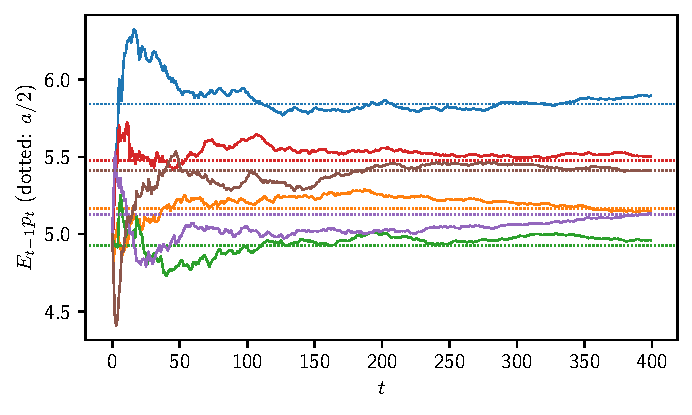
\includegraphics[width=.7\textwidth]{fig/ls02_23_monopolist.pdf}
\captionof{figure}{Exercise 2.23: $E_{t-1}p_t$ along six sample paths, each converging to its own $a/2$ (dotted).}\label{fig:mono}
\end{center}

%======================================================================
\subsection{The LQ Permanent Income Model and Howard Improvement}
%======================================================================

%------- 2.13 -------
\begin{tcolorbox}[oddbox,title={Exercise 2.13 \quad Permanent Income by Howard Improvement}]
\begin{tcolorbox}[questionbox]
A household has preferences over consumption processes $\{c_t\}_{t=0}^\infty$ that are ordered by
$-.5\sum_{t=0}^\infty\beta^t\left[(c_t-30)^2+.000001b_t^2\right]$ (1) where $\beta=.95$. The household
chooses a consumption, borrowing plan to maximize (1) subject to the sequence of budget constraints
$c_t+b_t=\beta b_{t+1}+y_t$ for $t\ge0$, where $b_0$ is an initial condition, $\beta^{-1}$ is the
one-period gross risk-free interest rate, $b_t$ is the household's one-period debt that is due in
period $t$, and $y_t$ is its labor income, which obeys the second-order autoregressive process
$(1-\rho_1L-\rho_2L^2)y_{t+1}=(1-\rho_1-\rho_2)5+.05w_{t+1}$ where $\rho_1=1.3,\rho_2=-.4$.\\[3pt]
(a) Define the \textit{state} of the household at $t$ as $x_t=[1\ b_t\ y_t\ y_{t-1}]'$ and the
\textit{control} as $u_t=(c_t-30)$. Then express the transition law facing the household in the form
(2.4.22). Compute the eigenvalues of $A$. Compute the zeros of the characteristic polynomial
$(1-\rho_1z-\rho_2z^2)$ and compare them with the eigenvalues of $A$. (\textit{Hint:} To compute the
zeros in Matlab, set $a=[.4\ -1.3\ 1]$ and call \texttt{roots(a)}. The zeros of $(1-\rho_1z-\rho_2z^2)$
equal the \textit{reciprocals} of the eigenvalues of the associated $A$.)\\
(b) Write a Matlab program that uses the Howard improvement algorithm (2.4.30) to compute the
household's optimal decision rule for $u_t=c_t-30$. Tell how many iterations it takes for this to
converge (also tell your convergence criterion).\\
(c) Use the household's optimal decision rule to compute the law of motion for $x_t$ under the optimal
decision rule in the form $x_{t+1}=(A-BF^*)x_t+Cw_{t+1}$, where $u_t=-F^*x_t$ is the optimal decision
rule. Using Matlab, compute the impulse response function of $[c_t\ b_t]'$ to $w_{t+1}$. Compare these
with the theoretical expressions (2.12.18).
\end{tcolorbox}

\textbf{Solution:}

\begin{enumerate}
\item From the budget constraint, $b_{t+1}=\beta^{-1}(c_t+b_t-y_t)=\beta^{-1}(30+b_t-y_t+u_t)$; income
is $y_{t+1}=(1-1.3+.4)5+1.3y_t-.4y_{t-1}+.05w_{t+1}=.5+1.3y_t-.4y_{t-1}+.05w_{t+1}$. So
$x_{t+1}=Ax_t+Bu_t+Cw_{t+1}$ with
\[
A=\begin{bmatrix}1&0&0&0\\30/\beta&1/\beta&-1/\beta&0\\.5&0&1.3&-.4\\0&0&1&0\end{bmatrix},\quad
B=\begin{bmatrix}0\\1/\beta\\0\\0\end{bmatrix},\quad
C=\begin{bmatrix}0\\0\\.05\\0\end{bmatrix},
\]
and the loss $\sum\beta^t(x_t'Rx_t+u_t'Qu_t)$ with $R=10^{-6}e_2e_2'$, $Q=1$ (the factor $.5$ is
irrelevant). $A$ is block triangular, so its eigenvalues are $1$ (constant), $1/\beta=1.052632$
(debt), and the roots of $\lambda^2-1.3\lambda+.4=0$: $\lambda=\frac{1.3\pm\sqrt{1.69-1.6}}{2}
=\frac{1.3\pm.3}2=\boxed{.8,\ .5}$. The zeros of $1-1.3z+.4z^2$ are
$z=\frac{1.3\pm.3}{.8}=\boxed{2,\ 1.25}$, the reciprocals of $.5$ and $.8$, as the hint says.
\item Howard (2.4.30): $P_j=R+F_j'QF_j+\beta(A-BF_j)'P_j(A-BF_j)$ (a Lyapunov equation in
$\sqrt\beta(A-BF_j)$, solved by doubling), $F_{j+1}=\beta(Q+\beta B'P_jB)^{-1}B'P_jA$. $A$ is unstable
($1/\beta$), so the initial rule must stabilise $\sqrt\beta(A-BF_0)$; we use the permanent-income slope
on debt, $F_0=[0,\ 1-\beta,\ 0,\ 0]$, which sets the closed-loop debt root to $1$. Convergence
criterion $\max|F_{j+1}-F_j|<10^{-10}$: \textbf{4 iterations}, and
\[
\begin{gathered}
F^*=[26.230541,\ .050019,\ -.396944,\ .150836],\\
c_t=30-F^*x_t=3.7695-.050019\,b_t+.396944\,y_t-.150836\,y_{t-1}.
\end{gathered}
\]
Compare the PIH rule (2.12.9): coefficient $-(1-\beta)=-.05$ on $b_t$, and on $(y_t,y_{t-1})$,
$(1-\beta)U_y(I-\beta A_{22})^{-1}$ with $A_{22}=\begin{bmatrix}1.3&-.4\\1&0\end{bmatrix}$:
$\det(I-\beta A_{22})=-.235+.361=.126$, first row of the inverse $[1,-.38]/.126=[7.93651,-3.01587]$,
times $.05$: $[.396825,-.150794]$. The tiny debt penalty moves them only in the fourth digit.
\item Closed loop $A-BF^*$ has eigenvalues $.5,\ .8,\ .99998,\ 1$: debt has a near-unit root (it
would be exactly 1 without the $10^{-6}$ penalty). Impulse responses to $w_{t+1}=1$:
$c_{t+1+j}$ responds by $-F^*(A-BF^*)^jC$ and $b_{t+1+j}$ by $e_2'(A-BF^*)^jC$. Theory (2.12.18):
\[
\begin{gathered}
d(\beta)=U_y(I-\beta A_{22})^{-1}C_2=\frac{.05}{1-1.3(.95)+.4(.95)^2}=\frac{.05}{.126}=.396825,\\
c:\ (1-\beta)d(\beta)=\boxed{.019841}\ \text{for all }j,
\end{gathered}
\]
\[
b_{t+1+j}:\ U_y(I-\beta A_{22})^{-1}A_{22}^{\,j}C_2-d(\beta)\quad(=0,\,-.031746,\,-.080952,\,-.132222,\dots).
\]
Numerically, $c$ jumps by $.019847$ and stays there (a box), and $b$ follows
$0,-.03174,-.08094,-.13220,\dots$, matching theory to about $.03\%$ (Figure~\ref{fig:irf13}). A
positive income shock raises consumption by the annuity value of the revised income forecast; since
the AR(2) makes income rise further before decaying, the household saves (debt falls), and the fall
in debt is permanent.
\end{enumerate}

\textbf{Verification.} \nb{2.13}: Howard's $F^*$ equals the Riccati solution from
\texttt{scipy.linalg.solve\_discrete\_are}; impulse responses agree with (2.12.18) within 2\% over 20
periods. \checkmark
\end{tcolorbox}

\begin{center}
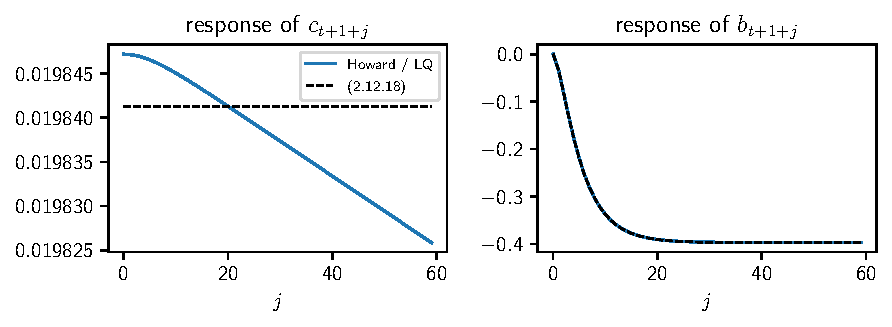
\includegraphics[width=\textwidth]{fig/ls02_13_irf.pdf}
\captionof{figure}{Exercise 2.13: impulse responses of consumption and debt to $w_{t+1}$, Howard/LQ
solution against formula (2.12.18).}\label{fig:irf13}
\end{center}

%------- 2.25 -------
\begin{tcolorbox}[oddbox,title={Exercise 2.25 \quad Consumption: the Two Classic Examples}]
\begin{tcolorbox}[questionbox]
(a) Please use formulas (2.12.18) to verify formulas (2.12.21) and (2.12.23)--(2.12.24) of subsection
2.12.3.\\
(b) Please use formulas (2.10.3) to compute the decision rules in formulas (2.12.21) and (2.12.23)
for the following parameter values: $\beta=.95,\sigma_1=\sigma_2=1$.\\
(c) Please use formulas (2.10.3) to compute the decision rules in formulas (2.12.21) and (2.12.23)
for the following parameter values: $\beta=.95,\sigma_1=2,\sigma_2=1$.\\
(d) Please use formula (2.12.20) to confirm formulas (2.12.22) and (2.12.25).
\end{tcolorbox}

\textbf{Solution:}

(2.12.18a) says $c_{t+1}-c_t=(1-\beta)U_y(I-\beta A_{22})^{-1}C_2w_{t+1}$.
\begin{enumerate}
\item \emph{Example 1}: $A_{22}=\text{diag}(1,0)$, $C_2=\text{diag}(\sigma_1,\sigma_2)$, $U_y=[1,1]$.
$(I-\beta A_{22})^{-1}=\text{diag}\big(\frac1{1-\beta},1\big)$, so
$U_y(I-\beta A_{22})^{-1}C_2=\big[\frac{\sigma_1}{1-\beta},\ \sigma_2\big]$, and
\[
c_{t+1}-c_t=(1-\beta)\Big[\tfrac{\sigma_1}{1-\beta}w_{1t+1}+\sigma_2w_{2t+1}\Big]=\sigma_1w_{1t+1}+(1-\beta)\sigma_2w_{2t+1}.\quad\text{(2.12.21)}\ \checkmark
\]
\emph{Example 2}: $z_t=[y_t,a_t]'$, $A_{22}=\begin{bmatrix}1&-(1-K)\\0&0\end{bmatrix}$,
$C_2=\begin{bmatrix}1\\1\end{bmatrix}$, $U_y=[1,0]$.
$I-\beta A_{22}=\begin{bmatrix}1-\beta&\beta(1-K)\\0&1\end{bmatrix}$, with inverse
$\begin{bmatrix}\frac1{1-\beta}&-\frac{\beta(1-K)}{1-\beta}\\0&1\end{bmatrix}$. Then
$U_y(I-\beta A_{22})^{-1}C_2=\frac{1-\beta(1-K)}{1-\beta}$ and
\[
c_{t+1}-c_t=[1-\beta(1-K)]\,a_{t+1}.\quad\text{(2.12.23)}\ \checkmark
\]
(2.12.18d) row 1: $y_{t+1}=y_t-(1-K)a_t+a_{t+1}$, i.e.\ $y_{t+1}-y_t=a_{t+1}-(1-K)a_t$ (2.12.24) \checkmark.
\item[(b,c)] \emph{Mapping to Muth.} $y_t=z_{1t}+z_{2t}$ with $z_{1,t+1}=z_{1t}+\sigma_1w_{1,t+1}$ and
$z_{2t}=\sigma_2w_{2t}$ iid: Muth's model (2.10.2) with $Q=\sigma_1^2$, $R=\sigma_2^2$. The fixed point
of (2.10.3b), $\Sigma=\Sigma+Q-\frac{\Sigma^2}{\Sigma+R}$, gives $\Sigma^2=Q(\Sigma+R)$, so
\[
\Sigma=\frac{Q+\sqrt{Q^2+4QR}}{2},\qquad K=\frac{\Sigma}{\Sigma+R},\qquad \Var(a_t)=\Sigma+R.
\]
\begin{center}\small
\setlength{\tabcolsep}{4pt}
\begin{tabular}{@{}lcccccc@{}}
\toprule
 & Ex.\,1: $\Delta c_{t+1}$ & $\Sigma$ & $K$ & $\Var(a)$ & Ex.\,2: $\Delta c_{t+1}$ & Ex.\,2: $\Delta b_{t+1}$\\
\midrule
(b) & $w_{1t+1}+.05w_{2t+1}$ & $1.618034$ & $.618034$ & $2.618034$ & $.637132\,a_{t+1}$ & $-.381966\,a_t$\\
(c) & $2w_{1t+1}+.05w_{2t+1}$ & $4.828427$ & $.828427$ & $5.828427$ & $.837006\,a_{t+1}$ & $-.171573\,a_t$\\
\bottomrule
\end{tabular}
\end{center}
Here $\Delta c_{t+1}=c_{t+1}-c_t$ and $\Delta b_{t+1}=b_{t+1}-b_t$; row (b) has $\sigma_1=\sigma_2=1$
and $\Sigma=\frac{1+\sqrt5}{2}$, row (c) has $\sigma_1=2,\sigma_2=1$ and $\Sigma=2+2\sqrt2$.
Arithmetic for (b): $K=\frac{1.618034}{2.618034}=.618034$, $1-\beta(1-K)=1-.95(.381966)=.637132$. For
(c): $Q=4$, $\Sigma^2-4\Sigma-4=0\Rightarrow\Sigma=2+2\sqrt2$; $K=\frac{4.828427}{5.828427}=.828427$;
$1-.95(.171573)=.837006$. A larger permanent variance makes the consumer attribute more of each
surprise to the permanent component, so consumption responds more and less is saved.
\item[(d)] (2.12.20): $b_{t+1}-b_t=U_y(I-\beta A_{22})^{-1}(A_{22}-I)z_t$.
\emph{Example 1}: $\big[\frac1{1-\beta},1\big]\text{diag}(0,-1)z_t=-z_{2t}=-\sigma_2w_{2t}$ (2.12.22) \checkmark.
\emph{Example 2}: $A_{22}-I=\begin{bmatrix}0&-(1-K)\\0&-1\end{bmatrix}$, and
$\big[\frac1{1-\beta},-\frac{\beta(1-K)}{1-\beta}\big](A_{22}-I)=\big[0,\ \frac{-(1-K)+\beta(1-K)}{1-\beta}\big]=[0,\ -(1-K)]$,
so $b_{t+1}-b_t=(K-1)a_t$ (2.12.25) \checkmark.
\end{enumerate}

\textbf{Verification.} \nb{2.25}: $A_{22},C_2$ run through (2.12.18) numerically; Riccati iteration
gives the same $K$; the innovations form reproduces the autocovariances of $\Delta y$:
$\Var(a)(1+(1-K)^2)=\sigma_1^2+2\sigma_2^2$ and $-(1-K)\Var(a)=-\sigma_2^2$. \checkmark
\end{tcolorbox}

%------- 2.27 -------
\begin{tcolorbox}[oddbox,title={Exercise 2.27 \quad Permanent Income Model Again}]
\begin{tcolorbox}[questionbox]
Each of two consumers named $i=1,2$ has preferences over consumption streams that are ordered by the
utility functional $E_0\sum_{t=0}^\infty\beta^tu(c^i_t)$ (1) where $E_t$ is the mathematical
expectation conditioned on the consumer's time $t$ information, $c^i_t$ is time $t$ consumption of
consumer $i$ at time $t$, $u(c)$ is a strictly concave one-period utility function, and
$\beta\in(0,1)$ is a discount factor. The consumer maximizes (1) by choosing a consumption, borrowing
plan $\{c^i_t,b^i_{t+1}\}_{t=0}^\infty$ subject to the sequence of budget constraints
$c^i_t+b^i_t=R^{-1}b^i_{t+1}+y^i_t$ where $y_t$ is an exogenous stationary endowment process, $R$ is a
constant gross risk-free interest rate, $b^i_t$ is one-period risk-free debt maturing at $t$, and
$b^i_0=0$ is a given initial condition. Assume that $R^{-1}=\beta$. We impose the following condition
on the consumption, borrowing plan of consumer $i$: $E_0\sum_{t=0}^\infty\beta^t(b^i_t)^2<+\infty$.
Assume the quadratic utility function $u(c_t)=-.5(c_t-\gamma)^2$, where $\gamma>0$ is a bliss level of
consumption. Negative consumption rates are allowed. Let $s_t\in\{0,1\}$ be an i.i.d.\ process with
$\text{Prob}(s_t=1)=\text{Prob}(s_1=0)=.5$. The endowment process of consumer 1 is $y^1_t=1-.5s_t$ and
the endowment process of person 2 is $y^2_t=.5+.5s_t$. Thus, the two consumers' endowment processes are
perfectly negatively correlated i.i.d.\ processes with means of .75.\\[3pt]
(a) Find optimal decision rules for consumption for both consumers. Prove that the consumers' optimal
decisions imply the following laws of motion for $b^1_t,b^2_t$:
$b^1_{t+1}(s_t=0)=b^1_t-.25$, $b^1_{t+1}(s_t=1)=b^1_t+.25$, $b^2_{t+1}(s_t=0)=b^2_t+.25$,
$b^2_{t+1}(s_t=1)=b^2_t-.25$.\\
(b) Show that for each consumer, $c^i_t,b^i_t$ are co-integrated.\\
(c) Verify that $b^i_{t+1}$ is risk-free in the sense that conditional on information available at
time $t$, it is independent of news arriving at time $t+1$.\\
(d) Verify that with the initial conditions $b^1_0=b^2_0=0$, the following two equalities obtain:
$b^1_t+b^2_t=0\ \forall t\ge1$, $c^1_t+c^2_t=1.5\ \forall t\ge1$. Use these conditions to interpret the
decision rules that you have computed as describing a closed pure consumption loans economy in which
consumers 1 and 2 borrow and lend with each other and in which the risk-free asset is a one-period IOU
from one of the consumers to the other.\\
(e) Define the `stochastic discount factor of consumer $i$' as $m^i_{t+1}=\frac{\beta u'(c^i_{t+1})}{u'(c^i_t)}$.
Show that the stochastic discount factors of consumer 1 and 2 are
$m^1_{t+1}=\beta+.25\frac{\beta(1-\beta)}{(\gamma-c^1_t)}$ if $s_{t+1}=0$, $\beta-.25\frac{\beta(1-\beta)}{(\gamma-c^1_t)}$
if $s_{t+1}=1$; $m^2_{t+1}=\beta-.25\frac{\beta(1-\beta)}{(\gamma-c^2_t)}$ if $s_{t+1}=0$,
$\beta+.25\frac{\beta(1-\beta)}{(\gamma-c^2_t)}$ if $s_{t+1}=1$. Are the stochastic discount factors of the
two consumers equal?\\
(f) Verify that $E_tm^1_{t+1}=E_tm^2_{t+1}=\beta$.
\end{tcolorbox}

\textbf{Solution:}

\begin{enumerate}
\item Apply (2.12.9), $c_t=(1-\beta)\big[\sum_{j\ge0}\beta^jE_ty_{t+j}-b_t\big]$. With iid endowments,
$E_ty^i_{t+j}=.75$ for $j\ge1$, so $\sum_j\beta^jE_ty^i_{t+j}=y^i_t+\frac{.75\beta}{1-\beta}$ and
\[
\boxed{c^i_t=(1-\beta)(y^i_t-b^i_t)+.75\beta}.
\]
Substituting into the budget constraint $b^i_{t+1}=\beta^{-1}(c^i_t+b^i_t-y^i_t)$:
\[
b^i_{t+1}=\beta^{-1}\big[(1-\beta)y^i_t-(1-\beta)b^i_t+.75\beta+b^i_t-y^i_t\big]
=\beta^{-1}\big[\beta b^i_t-\beta y^i_t+.75\beta\big]=b^i_t+.75-y^i_t .
\]
Consumer 1: $s_t=0\Rightarrow y^1_t=1\Rightarrow b^1_{t+1}=b^1_t-.25$; $s_t=1\Rightarrow y^1_t=.5\Rightarrow
b^1_{t+1}=b^1_t+.25$. Consumer 2: $s_t=0\Rightarrow y^2_t=.5\Rightarrow b^2_{t+1}=b^2_t+.25$;
$s_t=1\Rightarrow y^2_t=1\Rightarrow b^2_{t+1}=b^2_t-.25$. \checkmark
\item $b^i_{t+1}-b^i_t=.75-y^i_t$ is iid with mean zero: $b^i_t$ is a random walk, so it has a unit
root, and so does $c^i_t=(1-\beta)(y^i_t-b^i_t)+.75\beta$. But
\[
(1-\beta)b^i_t+c^i_t=(1-\beta)y^i_t+.75\beta
\]
is iid, hence stationary: $c^i_t,b^i_t$ are cointegrated with vector $[(1-\beta)\ \ 1]$, as in (2.12.19).
\item $b^i_{t+1}=b^i_t+.75-y^i_t$ is a function of $(b^i_t,s_t)$, known at $t$; it does not depend on
$s_{t+1}$ or on anything dated $t+1$. The payoff of the IOU is fixed when it is issued.
\item Summing the debt laws: $(b^1+b^2)_{t+1}-(b^1+b^2)_t=1.5-(y^1_t+y^2_t)=1.5-1.5=0$, so with
$b^1_0+b^2_0=0$, $\boxed{b^1_t+b^2_t=0}$ for all $t$. Then
$c^1_t+c^2_t=(1-\beta)(1.5-0)+1.5\beta=\boxed{1.5}$. Aggregate consumption equals the aggregate
endowment, which is constant. The economy is closed: whatever consumer 1 borrows, consumer 2 lends.
The only asset is a one-period IOU between them at gross rate $\beta^{-1}$, and it lets them smooth
each other's shocks.
\item $u'(c)=\gamma-c$, so $m^i_{t+1}=\beta\frac{\gamma-c^i_{t+1}}{\gamma-c^i_t}=\beta-\beta\frac{c^i_{t+1}-c^i_t}{\gamma-c^i_t}$.
From part a and the debt law,
$c^i_{t+1}-c^i_t=(1-\beta)\big[(y^i_{t+1}-y^i_t)-(b^i_{t+1}-b^i_t)\big]=(1-\beta)(y^i_{t+1}-.75)$. Consumer
1: $s_{t+1}=0\Rightarrow\Delta c^1=+.25(1-\beta)$; $s_{t+1}=1\Rightarrow\Delta c^1=-.25(1-\beta)$. Hence
\[
m^1_{t+1}=\begin{cases}\beta-.25\frac{\beta(1-\beta)}{\gamma-c^1_t},&s_{t+1}=0\\[3pt]
\beta+.25\frac{\beta(1-\beta)}{\gamma-c^1_t},&s_{t+1}=1\end{cases}\qquad
m^2_{t+1}=\begin{cases}\beta+.25\frac{\beta(1-\beta)}{\gamma-c^2_t},&s_{t+1}=0\\[3pt]
\beta-.25\frac{\beta(1-\beta)}{\gamma-c^2_t},&s_{t+1}=1\end{cases}
\]
These have the \textbf{opposite signs} to the printed statement (see the trap box). They are
\textbf{not equal}: in each state one consumer's SDF lies above $\beta$ and the other's below. With only
a risk-free bond, markets are incomplete, and the consumers cannot trade state-contingent claims that
would equate their marginal rates of substitution state by state.
\item $E_tm^1_{t+1}=.5\big(\beta-d^1_t\big)+.5\big(\beta+d^1_t\big)=\beta$ with
$d^1_t=.25\beta(1-\beta)/(\gamma-c^1_t)$; likewise for consumer 2. Both SDFs price the one asset that is
traded, the risk-free bond, at the common price $\beta=R^{-1}$. This is the Euler equation
$E_tu'(c_{t+1})=u'(c_t)$ in SDF form.
\end{enumerate}

\textbf{Verification.} \nb{2.27} ($\gamma=3$, 300 periods): debt laws, $b^1+b^2=0$, $c^1+c^2=1.5$, the
cointegrating residual, the SDF values $(.94475,\ .95525)$ for consumer 1, and $E_tm=\beta$. \checkmark
\end{tcolorbox}

\begin{tcolorbox}[trapbox]
The statement of 2.27(e) attaches ``$+$'' to $s_{t+1}=0$ for consumer 1. But $s_{t+1}=0$ is consumer
1's \emph{high}-endowment state ($y^1=1$): his consumption rises, his marginal utility $\gamma-c$ falls,
so $m^1_{t+1}<\beta$. The signs as printed would be right only if the endowment labels were swapped. The
answers to ``are they equal?'' (no) and to part f are unaffected.
\end{tcolorbox}

%------- 2.30 -------
\begin{tcolorbox}[evenbox,title={Exercise 2.30 \quad Phelps and Pollak (1968) Meet Howard}]
\begin{tcolorbox}[questionbox]
A sequence of decision makers at dates $t=0,1,\dots$, chooses $\{x_{t+1},u_t\}_{t=0}^\infty$ subject to
$x_{t+1}=Ax_t+Bu_t$, $t\ge0$ where $A$ is an $n\times n$ matrix, $B$ is an $n\times k$ matrix, $u_t$
is a $k\times1$ vector of time $t$ ``controls'', and $x_0$ is a given initial condition. Let
$r(x_t,u_t)=-(x_t'Rx_t+u_t'Qu_t)$, where $R$ and $Q$ are positive definite matrices. A time $t$
decision maker chooses $u_t,x_{t+1}$. A time $t$ decision maker's preferences are ordered by
$r(x_t,u_t)+\delta\sum_{j=1}^\infty\beta^jr(x_{t+j},u_{t+j})$ (0), where $\beta\in(0,1)$ and
$\delta\in(0,1]$.\\[3pt]
(a) Let $V(x)$ solve the following Bellman equation: $V(x)=r(x,-Fx)+\beta V((A-BF)x)$ (1). Please
interpret $V(x)$; i.e., please complete the sentence ``$V(x)$ is the value of \dots''.\\
(b) For a given matrix $F$, please guess a functional form for $V(x)$, then describe an algorithm for
solving the functional equation (1) for $V(x)$. Please get as far as you can in computing $V(x)$.\\
(c) Consider the functional equation $U(x)=\max_u\{r(x,u)+\delta\beta V(Ax+Bu)\}$ (2), where $V(x)$
satisfies the Bellman equation (1). Further, let $U(x)$ be attained by $u=-Gx$, so that
$U(x)=r(x,-Gx)+\delta\beta V((A-BG)x)$. Please interpret $U(x)$ as a value function.\\
(d) Please define a Markov perfect equilibrium for the sequence of problems solved by the sequence of
decision makers who choose $\{u_t\}_{t=0}^\infty$.\\
(e) Please describe how to compute a Markov perfect equilibrium in this setting.\\
(f) Please compare your algorithm for computing a Markov perfect equilibrium with the Howard policy
improvement algorithm.\\
(g) Let $\vec a_0=\{a_t\}_{t=0}^\infty$. Define $\vec a_1=\{a_t\}_{t=1}^\infty$ as the continuation of the
sequence $\vec a_0$. Is a continuation of a Markov perfect equilibrium a Markov perfect equilibrium?\\
(h) Suppose instead that there is a dictator who at time 0 chooses $\{u_t\}_{t=0}^\infty$ to maximize the
time $t=0$ value of the criterion (0). Please write Bellman equations and tell how to solve them for
an optimal plan for the time 0 dictator.\\
(i) Given $x_1$, a time 1 dictator chooses $\{u_t\}_{t=1}^\infty$ to maximize utility function (0) for
time $t$. Is a continuation of the time 0 dictator's plan the time 1 dictator's plan?\\
(j) Can you restrict $\delta\in(0,1]$ so that the time 0 dictator's plan equals the outcome of the
Markov perfect equilibrium that you described above?
\end{tcolorbox}

\textbf{Solution:}

\begin{enumerate}
\item Iterating (1), $V(x)=\sum_{j\ge0}\beta^jr(x_j,-Fx_j)$ with $x_{j+1}=(A-BF)x_j$, $x_0=x$.
\emph{$V(x)$ is the value of following the rule $u=-Fx$ forever from state $x$, discounted
exponentially at $\beta$, without the extra $\delta$.} It is the continuation value a current self
attaches, scaled by $\delta\beta$, to the path chosen by future selves who use $F$:
$r(x_t,u_t)+\delta\sum_{j\ge1}\beta^jr=r(x_t,u_t)+\delta\beta V(x_{t+1})$.
\item Guess $V(x)=-x'P_Fx$. Substituting into (1):
$-x'P_Fx=-x'(R+F'QF)x-\beta x'(A-BF)'P_F(A-BF)x$ for all $x$, so
\[
\boxed{P_F=R+F'QF+\beta(A-BF)'P_F(A-BF)},
\]
a discrete Lyapunov equation, i.e.\ (2.4.25). Algorithms: iterate $P_{k+1}=R+F'QF+\beta(A-BF)'P_k(A-BF)$
from $P_0=0$ (converges iff $\sqrt\beta(A-BF)$ is stable); or doubling; or in closed form
$\text{vec}(P_F)=\big[I-\beta(A-BF)'\otimes(A-BF)'\big]^{-1}\text{vec}(R+F'QF)$.
\item With $V=-x'P_Fx$ the maximand in (2) is $-x'Rx-u'Qu-\delta\beta(Ax+Bu)'P_F(Ax+Bu)$. First-order
condition: $-2Qu-2\delta\beta B'P_F(Ax+Bu)=0$, so
\[
u=-Gx,\qquad \boxed{G=\delta\beta\,(Q+\delta\beta B'P_FB)^{-1}B'P_FA}.
\]
\emph{$U(x)$ is the value, to the current self at state $x$, of choosing today's control optimally given
that all future selves will follow $u=-Fx$}, evaluated with the current self's quasi-hyperbolic
weights ($1$ today, $\delta\beta^j$ later). It is a one-shot deviation value, like (2.4.27).
\item A (stationary, linear) \textbf{Markov perfect equilibrium} is a rule $F$ such that, when every
future self uses $u=-Fx$, each current self's best response is also $u=-Fx$: $G(F)=F$, i.e.
\[
F=\delta\beta(Q+\delta\beta B'P_FB)^{-1}B'P_FA,\qquad P_F=R+F'QF+\beta(A-BF)'P_F(A-BF).
\]
Strategies depend only on the payoff-relevant state $x_t$, and the rule is a best response at every
date and every state.
\item Iterate on the pair: start from a stabilising $F_0$ (e.g.\ the $\delta=1$ optimum); given $F_j$,
solve the Lyapunov equation for $P_{F_j}$ (part b); set $F_{j+1}=\delta\beta(Q+\delta\beta B'P_{F_j}B)^{-1}B'P_{F_j}A$;
stop when $\max|F_{j+1}-F_j|<\varepsilon$. The limit satisfies both equations in (d).
\item It is Howard's algorithm (2.4.30) \textbf{with two discount factors}: the evaluation step uses
$\beta$ (future selves discount exponentially among themselves), the improvement step uses $\delta\beta$
(today's self discounts tomorrow more). With $\delta=1$ it \emph{is} (2.4.30). With $\delta<1$ the
iteration is a fixed-point search for a game equilibrium, not an optimisation, so Howard's monotone
improvement and convergence guarantees do not carry over. In the notebook example it converges in
10 ($\delta=.8$) and 14 ($\delta=.6$) iterations.
\item Yes. The MPE rule depends only on the current state and the problem at $t=1$ has the same
structure as at $t=0$, so the continuation $\{u_t=-Fx_t\}_{t\ge1}$ from any $x_1$ is again an MPE.
The equilibrium is subgame perfect by construction.
\item From date 1 on, the dictator's objective $\delta\sum_{j\ge1}\beta^jr$ is proportional to an ordinary
exponentially discounted problem, so the continuation plan solves
\[
W(x)=\max_u\{r(x,u)+\beta W(Ax+Bu)\},\qquad W(x)=-x'P^*x,
\]
\[
\begin{gathered}
P^*=R+\beta A'P^*A-\beta^2A'P^*B(Q+\beta B'P^*B)^{-1}B'P^*A,\\
F^*=\beta(Q+\beta B'P^*B)^{-1}B'P^*A,
\end{gathered}
\]
solved e.g.\ by Howard iterations (2.4.30). The date-0 control solves
$J(x_0)=\max_{u_0}\{r(x_0,u_0)+\delta\beta W(Ax_0+Bu_0)\}$, whose first-order condition gives
$u_0=-F_0x_0$, $F_0=\delta\beta(Q+\delta\beta B'P^*B)^{-1}B'P^*A$. The plan is $u_0=-F_0x_0$ and
$u_t=-F^*x_t$ for $t\ge1$.
\item No (for $\delta<1$). The time-1 dictator applies the same reasoning shifted one period and
picks $u_1=-F_0x_1$, not the $u_1=-F^*x_1$ the time-0 dictator planned for him. Preferences (0) are
time inconsistent: today's self discounts between $t+1$ and $t+2$ at $\beta$, but when $t+1$ arrives
that same trade-off is discounted at $\delta\beta$.
\item Yes: $\delta=1$. Then $F_0=F^*$, the dictator's plan is time consistent, and the MPE fixed point
is $F^*$ itself (a single Howard step from $F^*$ returns $F^*$). For $\delta<1$ the three rules differ.
Example with $A=\begin{bmatrix}1.02&.1\\0&.9\end{bmatrix}$, $B=[1,.5]'$, $R=I$, $Q=1$, $\beta=.95$:
\begin{center}\small
\begin{tabular}{@{}lccc@{}}
\toprule
$\delta$ & MPE $F$ & dictator $F_0$ (date 0) & dictator $F^*$ ($t\ge1$)\\
\midrule
1 & $[.580578,\ .209347]$ & $[.580578,\ .209347]$ & $[.580578,\ .209347]$\\
.8 & $[.535287,\ .193215]$ & $[.534341,\ .192674]$ & $[.580578,\ .209347]$\\
.6 & $[.477215,\ .173063]$ & $[.471727,\ .170097]$ & $[.580578,\ .209347]$\\
\bottomrule
\end{tabular}
\end{center}
Present bias makes every self control less aggressively (smaller feedback), and the MPE differs from
both pieces of the dictator's plan.
\end{enumerate}

\textbf{Verification.} \nb{2.30}: the MPE satisfies $G(F)=F$; at $\delta=1$ it equals the
\texttt{solve\_discrete\_are} optimum; at $\delta<1$ it does not. \checkmark
\end{tcolorbox}

%======================================================================
\section*{Companion code}
\addcontentsline{toc}{section}{Companion code}
%======================================================================

Notebook: \texttt{Resolucao/ljungqvist\_sargent/ls\_ch02.ipynb}.

It reproduces every numerical result above (Python: \texttt{numpy}, \texttt{scipy}, \texttt{matplotlib}), executed end to end with outputs saved. Each
section checks its numbers against an independent route with \texttt{assert}.

\begin{center}
\begin{tabular}{@{}p{3.6cm}p{11.2cm}@{}}
\toprule
\textbf{Item} & \textbf{What it does} \\
\midrule
helpers & \texttt{doublej} (doubling for $X=AXA'+CC'$, works with the constant's unit root),
\texttt{kalman\_steady} (iterates (2.7.14) to its fixed point), \texttt{save\_pdf} (pgf backend,
lmodern + cmap, so figure text is Type 1 and copyable). \\
\S\,2.1--2.3, 2.10--2.12, 2.14, 2.16--2.18 & Markov-chain likelihoods, stationary distributions,
absorption probabilities, simulations, lake-model MoM/ML and a Monte Carlo of the asymptotic covariance. \\
\S\,2.4--2.6, 2.8, 2.9, 2.29 & Companion forms, Lyapunov and doubling, prediction and discounting formulas,
population regression vs.\ simulated OLS, Cagan equilibria, SDF pricing by Monte Carlo, Howard-style
Kalman filter. \\
\S\,2.7, 2.15 & \texttt{bigshow3} counterpart; Slutsky spectra and peak locations. \\
\S\,2.19--2.24, 2.26, 2.28 & Kalman filters (scalar, time-varying $G_t$, cross-products checked by
brute-force Gaussian conditioning), innovations representations, VAR inversion, Kolmogorov--Szeg\H{o}
check. \\
\S\,2.13, 2.25, 2.27, 2.30 & Howard iterations vs.\ \texttt{solve\_discrete\_are}, impulse responses vs.\
(2.12.18), the two classic examples, the two-consumer loans economy, Markov perfect equilibrium. \\
\texttt{fig/ls02\_*.pdf} & The seven figures used in this file. \\
\bottomrule
\end{tabular}
\end{center}

\end{document}
